\chapter{Umsetzung}
\label{cha:umsetzung}
Im Folgenden wird der \ac{HiFi}-Prototyp gemäß der Zielsetzung unter Kapitel \ref{sec:ziel-der-arbeit} umgesetzt. Die Umsetzung umfasst die dort konkret genannten Funktionen. Nutzern soll es möglich sein den Kontostand abzurufen und unter Verwendung von Vorlagen Überweisungen durchzuführen. Die Basis für die Implementierung bilden die dafür relevanten Ergebnisse aus der Konzeption unter Kapitel \ref{cha:konzeption}.\\
Die Implementierung jeder Komponente ist im jeweiligen Kapitel beschrieben. Dabei werden die verwendeten Technologien, Besonderheiten und Probleme erläutert. Da es in der Arbeit in erster Linie um die konzeptionellen Aspekte der Umsetzung geht, wird versucht auf die Darstellung von Quelltext zu verzichten. Sämtlicher Programmcode aller Komponenten ist auf der CD zu finden.\\
Vor der detaillierten Beschreibung der Umsetzung, wird an dieser Stelle noch der Name des Systems genannt. Dies ist kein zentraler Bestandteil der Arbeit, jedoch spielt er für das Starten des zu entwickelnden Alexa Skills (Invocation-Name) und auch für die Smartphone-App eine Rolle. Zunächst fällt die Wahl auf „finlexa“, eine Zusammensetzung aus „financial“ und „Alexa“. Das Problem dabei ist die Verwendung als Invocation-Name. Der Sprachbefehl zum Starten des Skills ist dann: 

\begin{center}
    „Alexa, starte finlexa“
\end{center}

Besser ist die zweite Wahl „Voice Bank“. Nicht nur der Sprachbefehl ist geeigneter, der Name sagt zudem aus, was die Anwendung bezweckt. Abbildung zeigt das dafür konstruierte Logo\footnote{Das Logo wurde von Isabella Thürauf entworfen.}.

\begin{figure}[h]
  \centering
  
\includegraphics[width=0.4\textwidth]{bilder/4_logo.png}
  \caption{Voice Bank Logo}
  \label{fig:voicebank-logo}
\end{figure}

\section{Vorüberlegungen}
\label{sec:umsetzung-vorueberlegung}
Als Voraussetzung für das Implementieren der Kontostand-Abfrage und der Transaktion via Vorlage, müssen weitere Stories aus \ref{sec:anhang-user-stories} umgesetzt werden. Das schließt nicht nur die Hilfe (1) und Eingabemöglichkeit der TAN (16) ein, welche als Teil des Skill-Servers agieren, auch die Folgenden gehören dazu:

\begin{itemize}
    \item \textbf{Profilverwaltung (2- 4) und Authentifizierung (5)}: Diese werden unter Verwendung des Sicherheits-Konzeptes aus Kapitel \ref{sec:sicherheits-konzept} umgesetzt. Dafür werden eine App und ein Backend entwickelt. Für das Speichern der Benutzerprofile ist dem Backend auch eine Datenbank anzubinden. Die App bildet das Frontend für deren Verwaltung. Außerdem können sich Nutzer für die Verwendung des Alexa Banking Skills über die App authentifizieren. 
    
    \item \textbf{Bankkonten-Anbindung (6- 9) und Wahl des Hauptkontos (9)}: Um den Kontostand abzufragen und Überweisungen durchzuführen müssen Benutzer ihre Konten zunächst an das System anbinden. Da das bereits genannte Sicherheits-Konzept ohnehin die Entwicklung einer App und eines Backends vorsieht, kann man diese auch für die Anbindung der Bankkonten nutzen. Ein registrierter und angemeldeter Benutzer soll seine Konten über die App mit dem System verbinden können. Dabei werden die für die Verwendung erforderlichen Informationen in der Datenbank gespeichert. Das Hauptkonto bestimmen die Nutzer ebenfalls über die App, indem eines der verknüpften Konten dafür ausgewählt wird. Da es sich hier um einen Prototypen handelt, werden die Bankkonten gemockt. Hierfür wird der in Kapitel \ref{sec:bankkonto-anbindung} beschriebene Dienst verwendet.
    
    \item \textbf{Verwaltung der Überweisungsvorlagen (10- 12)}: Ebenso wie die Konto-Anbindungen können Nutzer auch ihre Überweisungsvorlagen über die Smartphone-App verwalten. In der Datenbank werden die Vorlagen in Relation zum entsprechenden Benutzer gespeichert. 
\end{itemize}

Abbildung \ref{fig:umsetzung-komponenten} zeigt eine Komponentenübersicht, in der diese Überlegungen einfließen.\newpage

\begin{figure}[!htb]
    \centering
    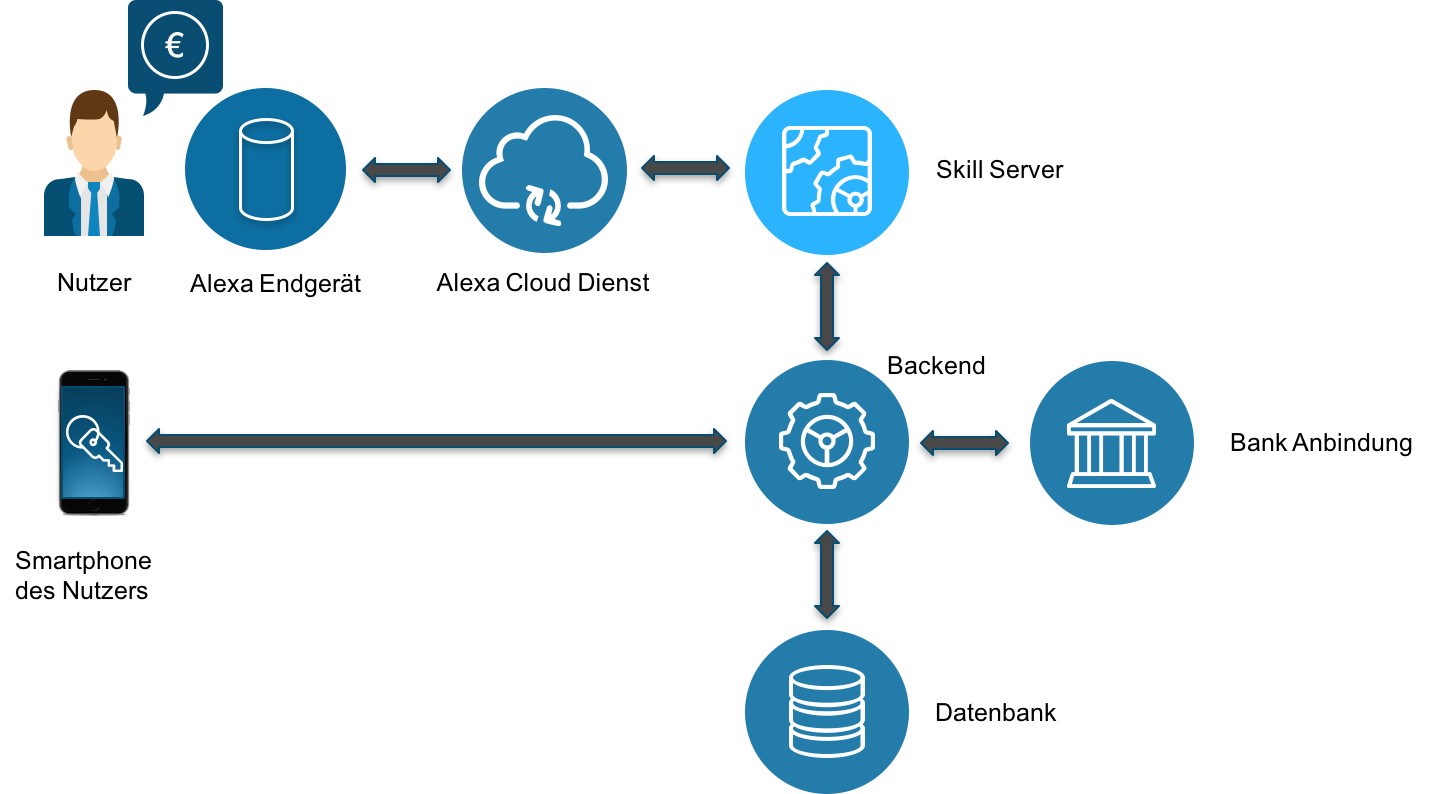
\includegraphics[width=1.0\textwidth]{bilder/4_umsetzungKomponenten.png}
    \caption{Komponentenübersicht für die Umsetzung}
    \label{fig:umsetzung-komponenten}
\end{figure}

Wie bereits erwähnt, speichert die Datenbank Benutzerprofile, Überweisungs-Vorlagen und Bankkonten-Anbindungen. Zunächst werden die dafür benötigten Datenmodelle beschrieben. Abbildung \ref{fig:datenbank-modell} zeigt eine vereinfachte Darstellung.

\begin{figure}[!htb]
    \centering
    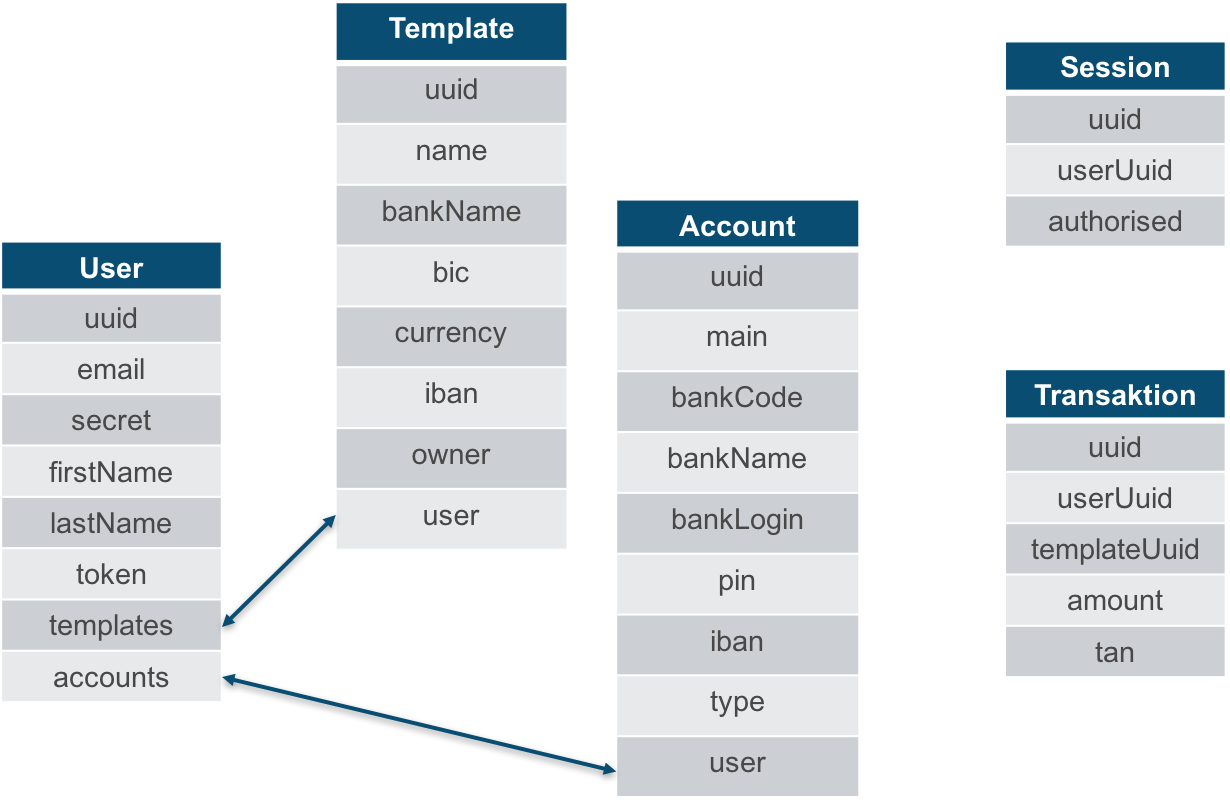
\includegraphics[width=0.8\textwidth]{bilder/4_datenmodelle.png}
    \caption{Vereinfachte Darstellung der Objekte und Relationen für die Datenbank}
    \label{fig:datenbank-modell}
\end{figure}

Jedes der Modelle hat einen \textit{\ac{UUID}}, um die Datensätze eindeutig zu kennzeichnen. Für ein Benutzerprofil sind nicht nur die Anmeldedaten wichtig, wie hier die Email Adresse und das Passwort (Secret). Der Vorname wird benötigt, um die Authentifizierung via Alexa für diesen anzustoßen. Für den Fall, dass Benutzer den gleichen Vornamen haben dient der Nachname der Unterscheidung dieser Nutzer. Mit Hilfe des Tokens wird das Smartphone des hinterlegten Benutzers für die Push-Nachrichten adressiert. Diese werden in den Kapiteln \ref{sec:backend} und \ref{sec:app} genauer betrachtet. Außerdem gehören Templates und Accounts zum Benutzerprofil, welche mit den entsprechenden Datensätzen verknüpft sind. Dabei handelt es sich um die Überweisungs-Vorlagen und Bankkonten-Anbindungen, die dieser Nutzer angelegt hat. Eine Überweisungs-Vorlage enthält alle notwendigen Informationen für das Durchführen von Transaktionen über Alexa, darunter die Zielbank, \ac{BIC}, \ac{IBAN} des Zielkontos und der Kontoinhaber. Beim Anlegen der Vorlage muss der Benutzer einen Namen vergeben, um die Vorlage über Alexa zu adressieren. Der Betrag ist nicht Bestandteil der Vorlage, da dieser vom Benutzer über Sprache eingegeben wird.\\ 
Die Konto-Anbindung speichert ebenfalls die Daten für den Login, die für die Anmeldung bei der entsprechenden Online-Banking-Anwendung verwendet werden. Neben der \ac{IBAN} wird auch der Typ des Kontos gespeichert. Dieser kann vom Nutzer festgelegt werden und dient als Orientierungshilfe in der App. Das Feld „main“ sagt aus, ob es sich bei diesem Konto um das Hauptkonto handelt. Auch die Konto-Anbindung verweist auf den Benutzer, der die Verknüpfung angelegt hat.\\
Die Datenbank wird entsprechend dieser Modelle an das Backend angebunden. Das heißt, dass nur das Backend einen direkten Zugriff auf diese Daten hat. Damit auch andere Anwendungen auf die Daten zurückgreifen können, muss das Backend eine Schnittstelle zur Verfügung stellen, die von diesen Anwendungen konsumiert werden kann. Diese Schnittstelle wird zunächst modelliert.\\
Es gibt verschiedene Formen der Interoperabilität zwischen Diensten im Internet. Eine dieser Formen ist \ac{REST}. Da die Alexa Plattform mit dem Skill-Server via \ac{REST} kommuniziert, soll auch das Backend eine solche Schnittstelle bereit stellen. Tabelle \ref{tab:backend-rest-api} zeigt die modellierte \ac{REST}-Schnittstelle. Dabei werden die \textit{\ac{CRUD}} Operationen für Profile, Bank-Anbindungen und Überweisungs-Vorlagen umgesetzt. \ac{CRUD} definiert die vier Basis Operationen für persistenten Speicher. Einige der Endpunkte beinhalten geklammerte Ausdrücke, wie \zB „\{userId\}“. Diese stellen Parameter dar, die sich für jede Anfrage ändern können. Alle Id-Parameter sind Platzhalter für die \ac{UUID} des jeweiligen Datensatzes. 

\begin{table}[!h]
\centering
 \begin{tabular}{ | m{4.5cm} || C{2cm}| C{2cm} | C{2cm} | C{2cm} |} 
 \hline
 Ressource & POST & GET & PUT & DELETE\\ 
 Endpunkt & create & read & update & delete \\
 \hhline{=::====}
  /users & Profil anlegen & Alle Profile ausgeben & n.a. & n.a.\\ 
 \hline /users/\{userId\} & n.a. & Profil ausgeben & Profil bearbeiten & Profil löschen\\
 \hline /users/\{userId\}/accounts & Account anlegen & Alle Accounts des Nutzers ausgeben & n.a. & n.a.\\
 \hline /users/\{userId\}/accounts/\{accId\} & n.a. & Account ausgeben & Account bearbeiten & Account löschen\\
 \hline /users/\{userId\}/templates & Template anlegen & Alle Templates des Nutzers ausgeben & n.a. & n.a.\\ 
 \hline /users/\{userId\}/templates/
 \{tmpId\} & n.a. & Template ausgeben & Template bearbeiten & Template löschen\\ 
 \hline
\end{tabular}
\caption{Backend REST-Schnittstelle für die Verwaltung von Profilen, Bank-Anbindungen und Überweisung-Vorlagen}
\label{tab:backend-rest-api}
\end{table}

Die hier modellierte \ac{REST}-Schnittstelle für das Backend setzt in Verbindung mit der App die Stories für die Verwaltung von Profilen (2-4), Bank-Anbindungen (6-9) und Überweisungs-Vorlagen (10-12) um. Für die eigentlichen Banking Funktionalitäten über Alexa, darunter die Authentifizierung (5), Kontostand Abfrage (13), Transaktion (14) und TAN-Eingabe (16), muss der Skill-Server mit dem Backend kommunizieren. Auch für diese Kommunikation soll das Backend eine \ac{REST}-Schnittstelle definieren. Zunächst wird der Vorgang der Authentifizierung näher betrachtet. \\
Benötigt man für die Verwendung eines Alexa Skills zusätzliche Endgeräte, wie hier das Smartphone, sind gewisse Dinge zu beachten. Alexa funktioniert nach dem Frage-Antwort-Prinzip. Ein Benutzer stößt die Interaktion an und der Skill-Server gibt die Antwort zurück. Alexa kann dabei nicht über Ereignisse (engl. Events) gesteuert werden. Gemäß Kapitel \ref{sec:sicherheits-konzept} startet die Authentifizierung, sobald der Name des Benutzers eingegeben wird. Nun kann zwar die Aufforderung an das Smartphone des Nutzers gesendet werden, jedoch kann die Bestätigung des Fingerabdrucks nicht direkt die Ausgabe über Alexa anstoßen. Aus diesem Grund werden Session-Objekte verwendet. Sie werden vom Backend verwaltet und ebenfalls in der Datenbank gespeichert. Abbildung \ref{fig:datenbank-modell} zeigt auch das Modell der Session. Nennt ein Benutzer seinen Namen wird ein Session-Objekt im Backend \bzw der Datenbank angelegt und die Aufforderung zur Bestätigung des Fingerabdruckes an das mobile Endgerät geschickt. Für einen besseren Überblick wird im Folgenden das Zusammenspiel zwischen Skill-Server, Backend und App für den Authentifizierungsprozess dargestellt. Abbildung \ref{fig:sequenz-authentifizierung} zeigt diesen in Form eines Sequenzdiagrammes. 

\begin{figure}[!htb]
    \centering
    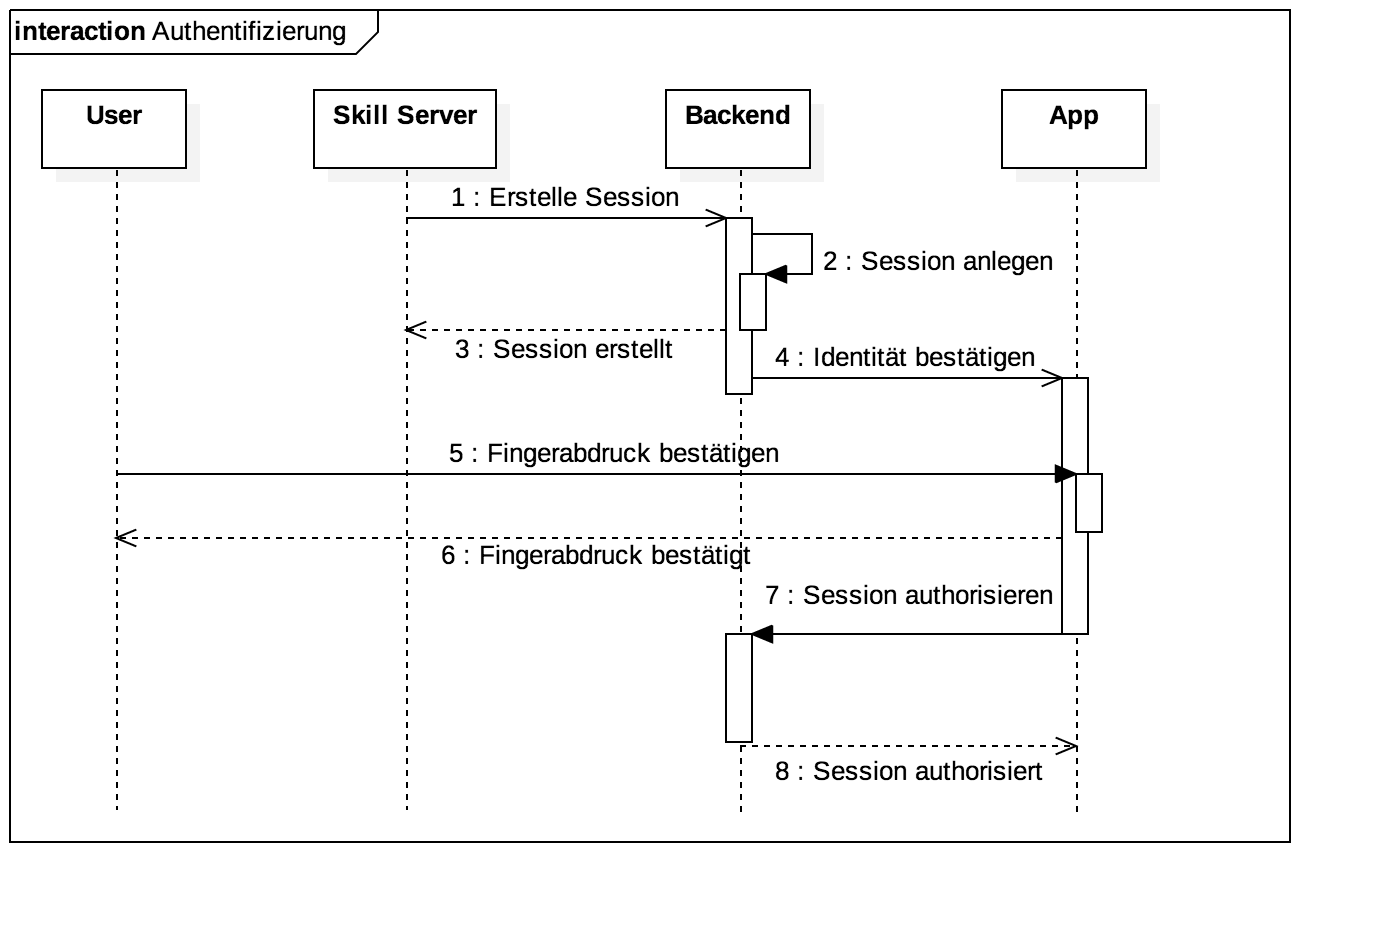
\includegraphics[width=1.0\textwidth]{bilder/4_sequenzAuthentifizierung.png}
    \caption{Sequenzdiagramm für den Authentifizierungsprozess}
    \label{fig:sequenz-authentifizierung}
\end{figure}

Bei erfolgreicher Authentifizierung teilt nun die App dem Backend mit, dass diese Session autorisiert ist. Im Anschluss können die Banking Funktionen über Alexa genutzt werden. Wird der Skill beendet ist die Authorisierung nichtig. Bei erneutem Öffnen muss der Vorgang wiederholt werden. Im Folgenden wird der Prozess der Kontostand-Abfrage betrachtet.\\
Ist die Session des Benutzers autorisiert, kann der Kontostand abgefragt werden. Da das Backend als Vermittler zwischen Skill-Server und Bank-Anbindung agiert (\vgl Abbildung \ref{fig:umsetzung-komponenten}), wird auch hierfür ein Endpunkt benötigt, der vom Skill-Server angesprochen werden kann. Bei Verwendung holt sich das Backend, über das vom Benutzer hinterlegte Hauptkonto die Information von der Bank-Anbindung. Abbildung \ref{fig:sequenz-kontostand} veranschaulicht den Prozess.\newpage

\begin{figure}[!htb]
    \centering
    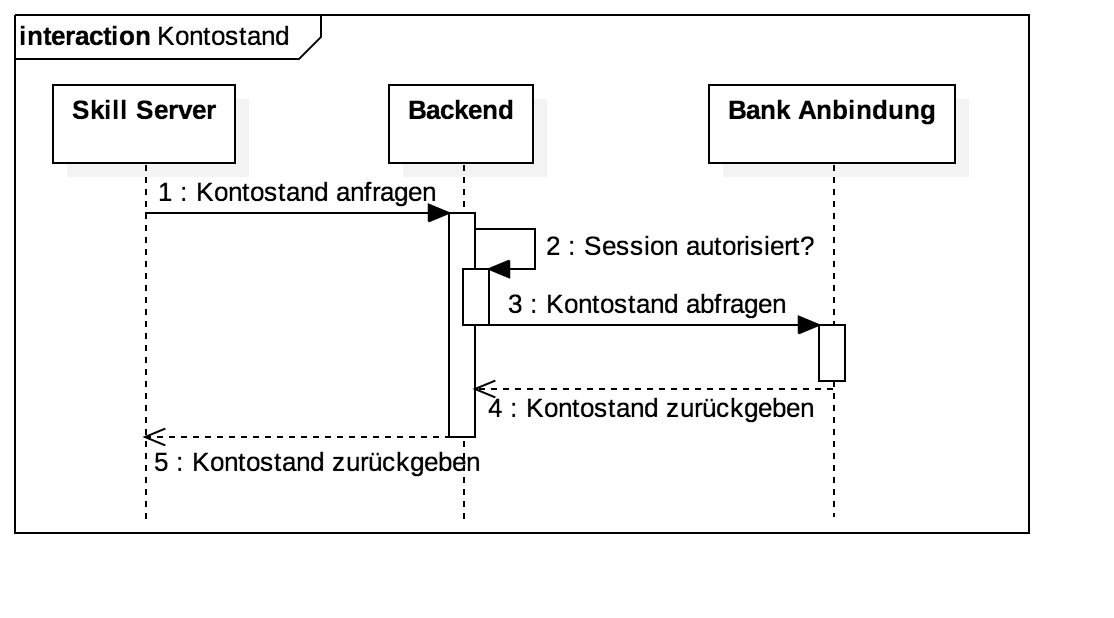
\includegraphics[width=1.0\textwidth]{bilder/4_sequenzKontostand.png}
    \caption{Sequenzdiagramm für die Abfrage des Kontostandes}
    \label{fig:sequenz-kontostand}
\end{figure}

Die Durchführung einer Transaktion ist ähnlich. Der Skill-Server sendet eine Anfrage mit den für die Überweisung benötigten Daten an das Backend. Anders als die Kontostand Abfrage muss eine Transaktion zusätzlich über die Eingabe einer \ac{TAN} bestätigt werden. Auch hier kann vorerst ein Objekt angelegt werden, welches sämtliche Informationen für die Durchführung der Überweisung enthält (\vgl Abbildung \ref{fig:datenbank-modell}). Darunter der Benutzer und die verwendete Überweisungsvorlage in Form der entsprechenden \acp{UUID}. Zusätzlich wird der Betrag für die Durchführung benötigt. Da es sich um einen Prototypen handelt und die Bankkonten gemockt werden, gibt es keine Bank für die Generierung der \ac{TAN}. Sie muss vom Backend erzeugt werden. Dieser Prozess wird in Abbildung \ref{fig:sequenz-transaktion-anlegen} veranschaulicht.\newpage

\begin{figure}[!htb]
    \centering
    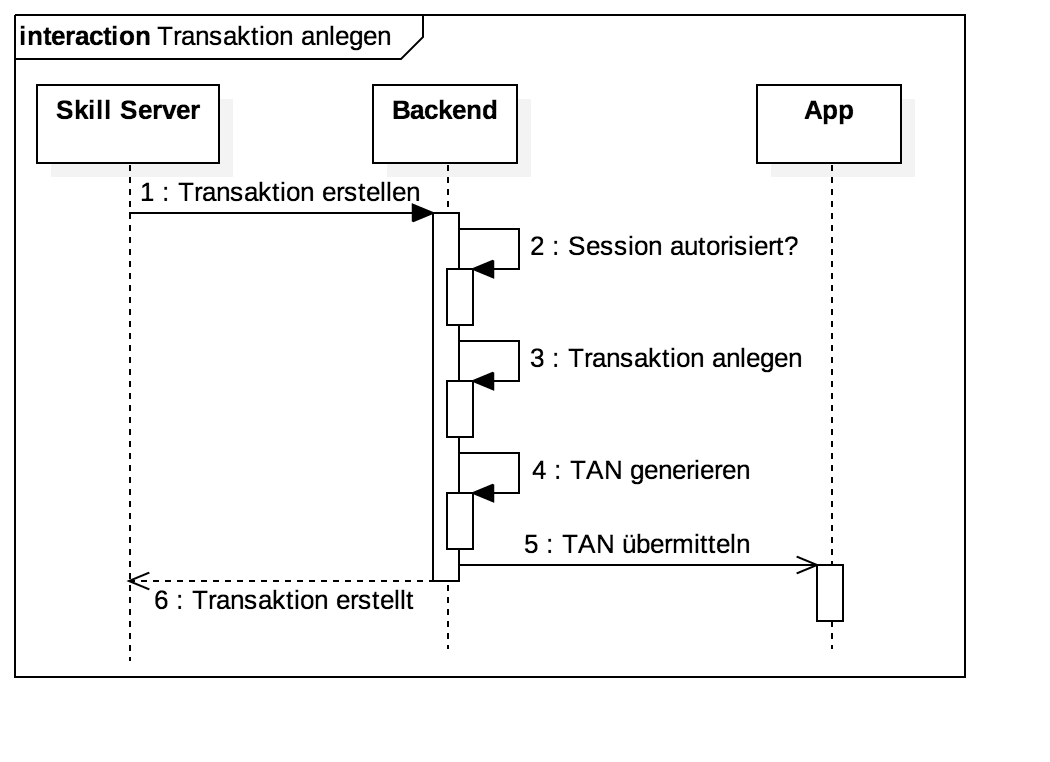
\includegraphics[width=1.0\textwidth]{bilder/4_sequenzTransaktionAnlegen.png}
    \caption{Sequenzdiagramm für das Anlegen einer Transaktion}
    \label{fig:sequenz-transaktion-anlegen}
\end{figure}

Im Anschluss wird dem Benutzer die Nummer per Smartphone-App übermittelt. Nachdem er die \ac{TAN} in den Echo diktiert hat wird diese validiert. Ist die Nummer korrekt wird die Transaktion bestätigt und an die Bank-Anbindung gesendet, zu sehen in Abbildung \ref{fig:sequenz-transaktion-bestaetigen}.\newpage 

\begin{figure}[!htb]
    \centering
    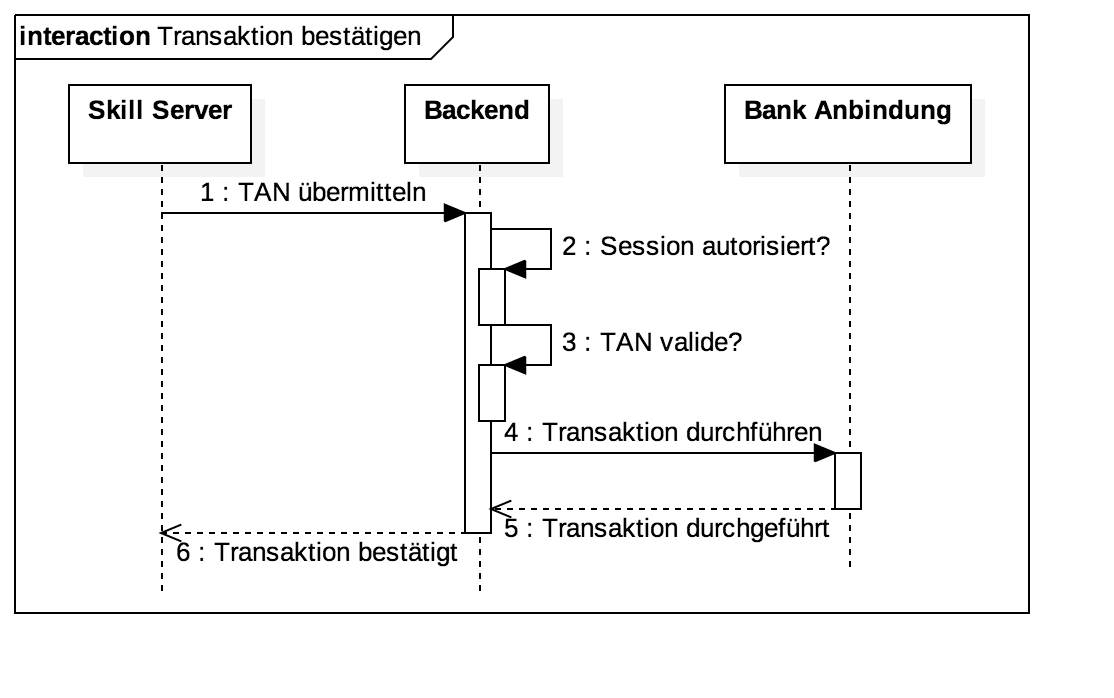
\includegraphics[width=1.0\textwidth]{bilder/4_sequenzTransaktionbestaetigen.png}
    \caption{Sequenzdiagramm für das Bestätigen einer Transaktion}
    \label{fig:sequenz-transaktion-bestaetigen}
\end{figure}

Das Diktieren der \ac{TAN} über den Echo ist dabei unkritisch, da diese Nummer nur einmal gültig ist.\\
Zusätzlich zur bereits gezeigten Schnittstelle benötigt das Backend also eine weitere für die Ausführung der beschriebenen Banking-Funktionen. Daraus ergibt sich das in Tabelle \ref{tab:backend-banking-rest-api} gezeigte Modell.

\begin{table}[!htb]
\centering
 \begin{tabular}{ | m{4cm} || C{2cm}| C{2cm} | C{2cm} | C{2cm} |} 
 \hline
 Ressource & POST & GET & PUT & DELETE\\ 
 Endpunkt & create & read & update & delete\\
 \hhline{=::====}
  /sessions & Session anlegen & Alle Sessions ausgeben & n.a. & n.a.\\ 
 \hline /sessions/\{sessionId\} & Session authorisieren & Session ausgeben & Autorisierung erneut senden & n.a.\\
 \hline /balance & Kontostand ausgeben & n.a. & n.a. & n.a.\\
\hline/transactions & Transaktion anlegen & Alle Transaktionen ausgeben & n.a. & n.a.\\ 
 \hline /transactions/\{transId\} & n.a. & Transaktion ausgeben & n.a. & n.a.\\ 
\hline /transactions/\{transId\}/\{tan\} & Transaktion bestätigen & n.a. & n.a. & n.a.\\ 
 \hline
\end{tabular}
\caption{Backend REST-Schnittstelle für Banking Funktionen}
\label{tab:backend-banking-rest-api}
\end{table}

Die folgenden Kapitel beschreiben die Implementierung jeder Komponente aus Abbildung \ref{fig:umsetzung-komponenten}. Der Fokus der Arbeit liegt auf der Umsetzung des \ac{CUI}. Aus diesem Grund werden die Kapitel des Skill-Servers (\ref{sec:skill-server}) und Interaction Models (\ref{sec:interaction-model}) detaillierter beschrieben. Für die anderen Kapitel soll lediglich ein Überblick gegeben werden. 

\section{Bank-Anbindung}
\label{sec:bankkonto-anbindung}
Da es sich bei der Umsetzung um einen Prototypen handelt, werden keine realen Konten an das System angebunden. Die Daten werden über den \textit{Multibanking-Mock-Service} simuliert. Dabei handelt es sich um einen bereits existierenden Dienst, der vom Projektträger der Arbeit bereit gestellt wird. Im weiteren Verlauf wird dieser als Multibank-Mock oder einfach nur Mock bezeichnet. Neben diesem gibt es auch den \textit{Multibanking-Service}. Darüber ist die Anbindung realer Konten möglich. Da die Datenmodelle beider Services ähnlich sind, ist eine spätere Integration des Multibanking-Service gut umzusetzen. Der Mock wird beim Projektträger verwendet, um entwickelte Anwendungen mit Kontodaten zu testen. Die Konten kann man dabei beliebig konfigurieren. Kontostände, Buchungen, Daueraufträge \usw können über die \ac{REST}-Schnittstelle des Mocks \bzw dem Hochladen einer Excel-Tabelle bequem eingerichtet und geändert werden. Da der Fokus der Arbeit ein anderer ist, werden hier Datenmodell und Endpunkte des Mocks nicht näher erläutert. Für den späteren Test des Prototypen wird mit dessen Hilfe ein Konto erstellt und an das System angebunden.

\section{Backend}
\label{sec:backend}
Das Backend ist die vermittelnde Instanz zwischen Skill-Server, Smartphone-App, Datenbank und Bank-Anbindung. Ein Teil der Funktionalität ist bereits in Kapitel \ref{sec:umsetzung-vorueberlegung} konzeptionell beschrieben. Die dort beschriebenen \ac{REST}-Schnittstellen und die Datenbank-Anbindung werden im Backend umgesetzt. Die Prozesse der Authentifizierung sehen außerdem vor, dass das Backend Informationen an die Smartphone-App übermittelt. Wie in Kapitel \ref{sec:sicherheits-konzept} erwähnt, soll dies über Push-Nachrichten erfolgen, daher ist auch diese Funktionalität im Backend zu implementieren. 

\subsection{Datenbank}
\label{subsec:backend-datenbank}
Als Datenbank aus Abbildung \ref{fig:umsetzung-komponenten} kommt \textit{PostgreSQL} \cite{postgres} zum Einsatz. Dabei handelt es sich um eine Open-Source \textit{\ac{SQL}} Datenbank. Für diese Wahl gibt es keinen bestimmten Grund.

\subsection{Plattform}
\label{backend-plattform}
Bei der Implementierung des Backends wird \textit{Node.js} \cite{node-js} verwendet, eine serverseitige \textit{\ac{JS}} Plattform. Da bei der Alexa Skill Entwicklung größtenteils darauf zurückgegriffen wird, ist der Skill-Server ebenfalls in Node.js entwickelt. Im Bereich des Backends gibt es jedoch keinen speziellen Grund dafür. Eine Node.js Anwendung kann über den \textit{\ac{npm}} \cite{npm}, mit zusätzlichen Open-Source Bibliotheken, sogenannten Modulen, erweitert werden. Auf die wichtigsten Bibliotheken wird im Folgenden eingegangen.

\begin{itemize}
    \item \textit{Express}: Express ist ein minimalistisches und flexibles Node.js Framework für Web-Anwendungen, dass vieles an Funktionalität mit sich bringt. Hier wird es in erster Linie für den Aufbau der Endpunkte, der Integration von \textit{Middleware}\footnote{Bei Web Servern handelt es sich dabei um Routinen, die zwischen dem Endpunkt und der eigentlichen Businesslogik greifen.} und dem Starten der Backend-Anwendung verwendet. Express erleichtert vor allem die Umsetzung der in Kapitel \ref{sec:umsetzung-vorueberlegung} beschriebenen \ac{REST}-Schnittstellen \cite{express-js}.
    
    \item \textit{\ac{TS}}: TypeScript ist ein typisiertes Superset von \ac{JS}. Es ermöglicht die Implementierung von Klassen und ist typensicher, was die ausschlaggebenden Gründe für die Verwendung sind. Der Quelltext des Backends und des Skill-Servers sind in \ac{TS} geschrieben. Für die Ausführung des Programmcodes wird der Quelltext vorher in \ac{JS} kompiliert \cite{typescript}. 
    
    \item \textit{TypeORM}: Dabei handelt es sich um ein Modul für \textit{\ac{ORM}}. Diese Technik wird im Allgemeinen dafür verwendet, Daten zwischen System mit inkompatiblen Typen zu transferieren. Im Backend wird \ac{ORM} für die Datenbank-Anbindung genutzt. Es erlaubt eine komfortable Verwaltung der Daten unter Verwendung bereits implementierter \ac{TS} Typen \bzw Klassen. Das Schreiben von \textit{\ac{SQL}} Methoden entfällt dabei \cite{typeorm}.
    
    \item \textit{Firebase}: Firebase ist eine freie Plattform, die bei der Entwicklung von mobilen Anwendungen unterstützt. Sie bietet dabei viele unterschiedliche Funktionen an. Hier wird lediglich das \textit{Cloud Messaging} verwendet, um die Push-Nachrichten für die Authentifizierung und das Versenden der \ac{TAN} umzusetzen. Um Firebase nutzen zu können, muss man sich zunächst registrieren und seine Anwendung hinterlegen. Das Backend agiert als der Server, der die Nachrichten über Firebase an die hinterlegte App schickt. Dafür ist im Backend die „Firebase Service“ Klasse implementiert. Für Nutzung des Dienstes, werden Daten aus dem Firebase Benutzerprofil benötigt. Um diese Daten bei Veröffentlichung der Arbeit zu schützen, wird der Teil des Quelltextes entfernt und entsprechend kommentiert \cite{firebase}.
\end{itemize}

Der Programmcode des Backends ist auf der beiliegenden CD unter \textit{„Quelltexte/finlexa\_central/“} zu finden.

\section{Smartphone Anwendung}
\label{sec:app}
Die App ist nicht nur ein wichtiger Teil des Sicherheits-Konzeptes, sondern bildet auch das Frontend für die Verwaltung der Profile, Überweisungsvorlagen und Bankkonten-Anbindungen. Auch hier soll nur ein Überblick gegeben und nicht im Detail auf den Quelltext eingegangen werden. Die App ist für das \textit{Android} Betriebssystem \cite{android} implementiert. Im Folgenden werden anhand der erstellten Oberflächen die grundlegenden Funktionen der Anwendung erklärt. Aufgrund der zeitlichen Begrenzung beschränkt sich die Anwendung in erster Linie auf die Funktionalität. Gestaltung und Usability liegt hier nicht im Fokus.

\subsection{Registrieren und anmelden}
\label{subsec:app-registrieren-anmelden}
Damit sich Benutzer registrieren können, wird die entsprechende \ac{REST}-Schnittstelle des Backends konsumiert. Abbildung \ref{fig:app-login} zeigt die Bildschirme für den Login-Bereich und der Registrierung. Letzterer wird durch Klicken des Buttons auf dem Login-Bildschirm geöffnet.

\begin{figure}[h]
  \centering
  \begin{minipage}[b]{0.45\textwidth}
    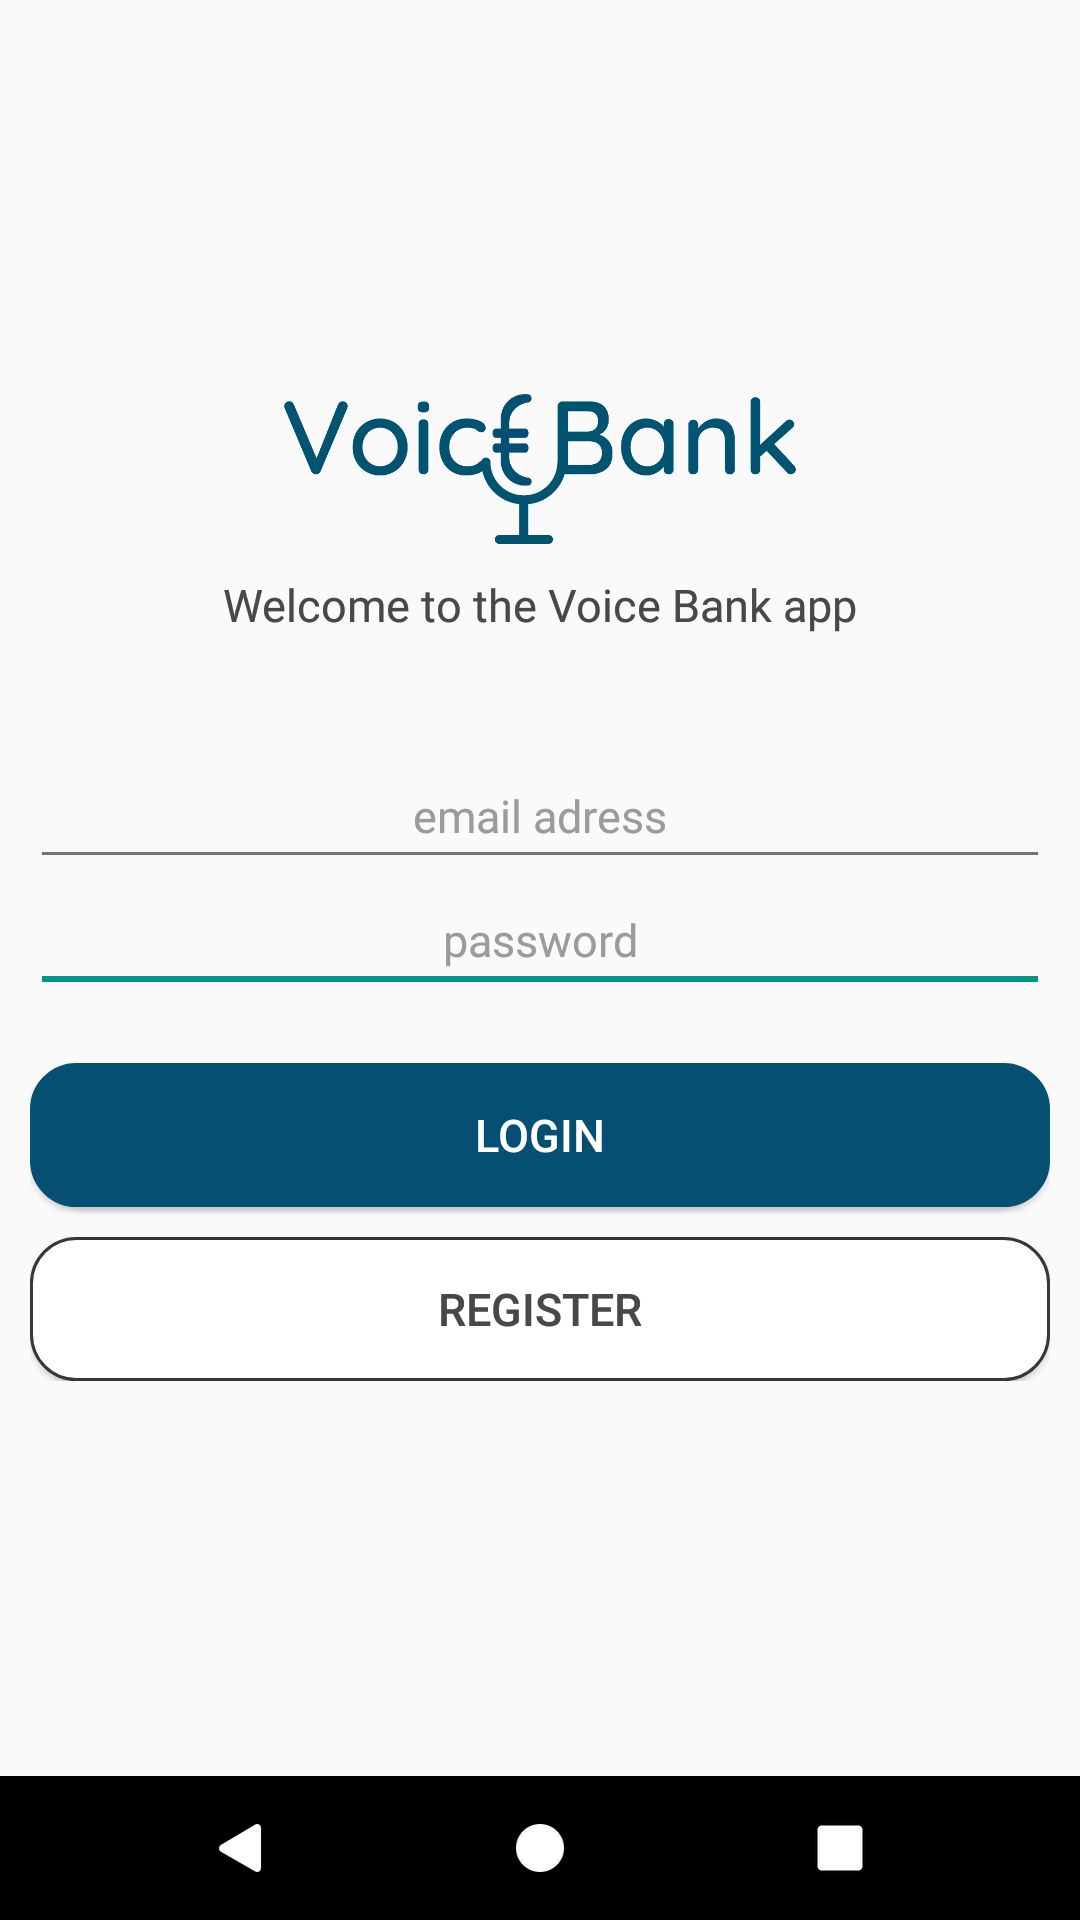
\includegraphics[width=\textwidth]{bilder/4_appLogin.png}
  \end{minipage}
  \begin{minipage}[b]{0.45\textwidth}
    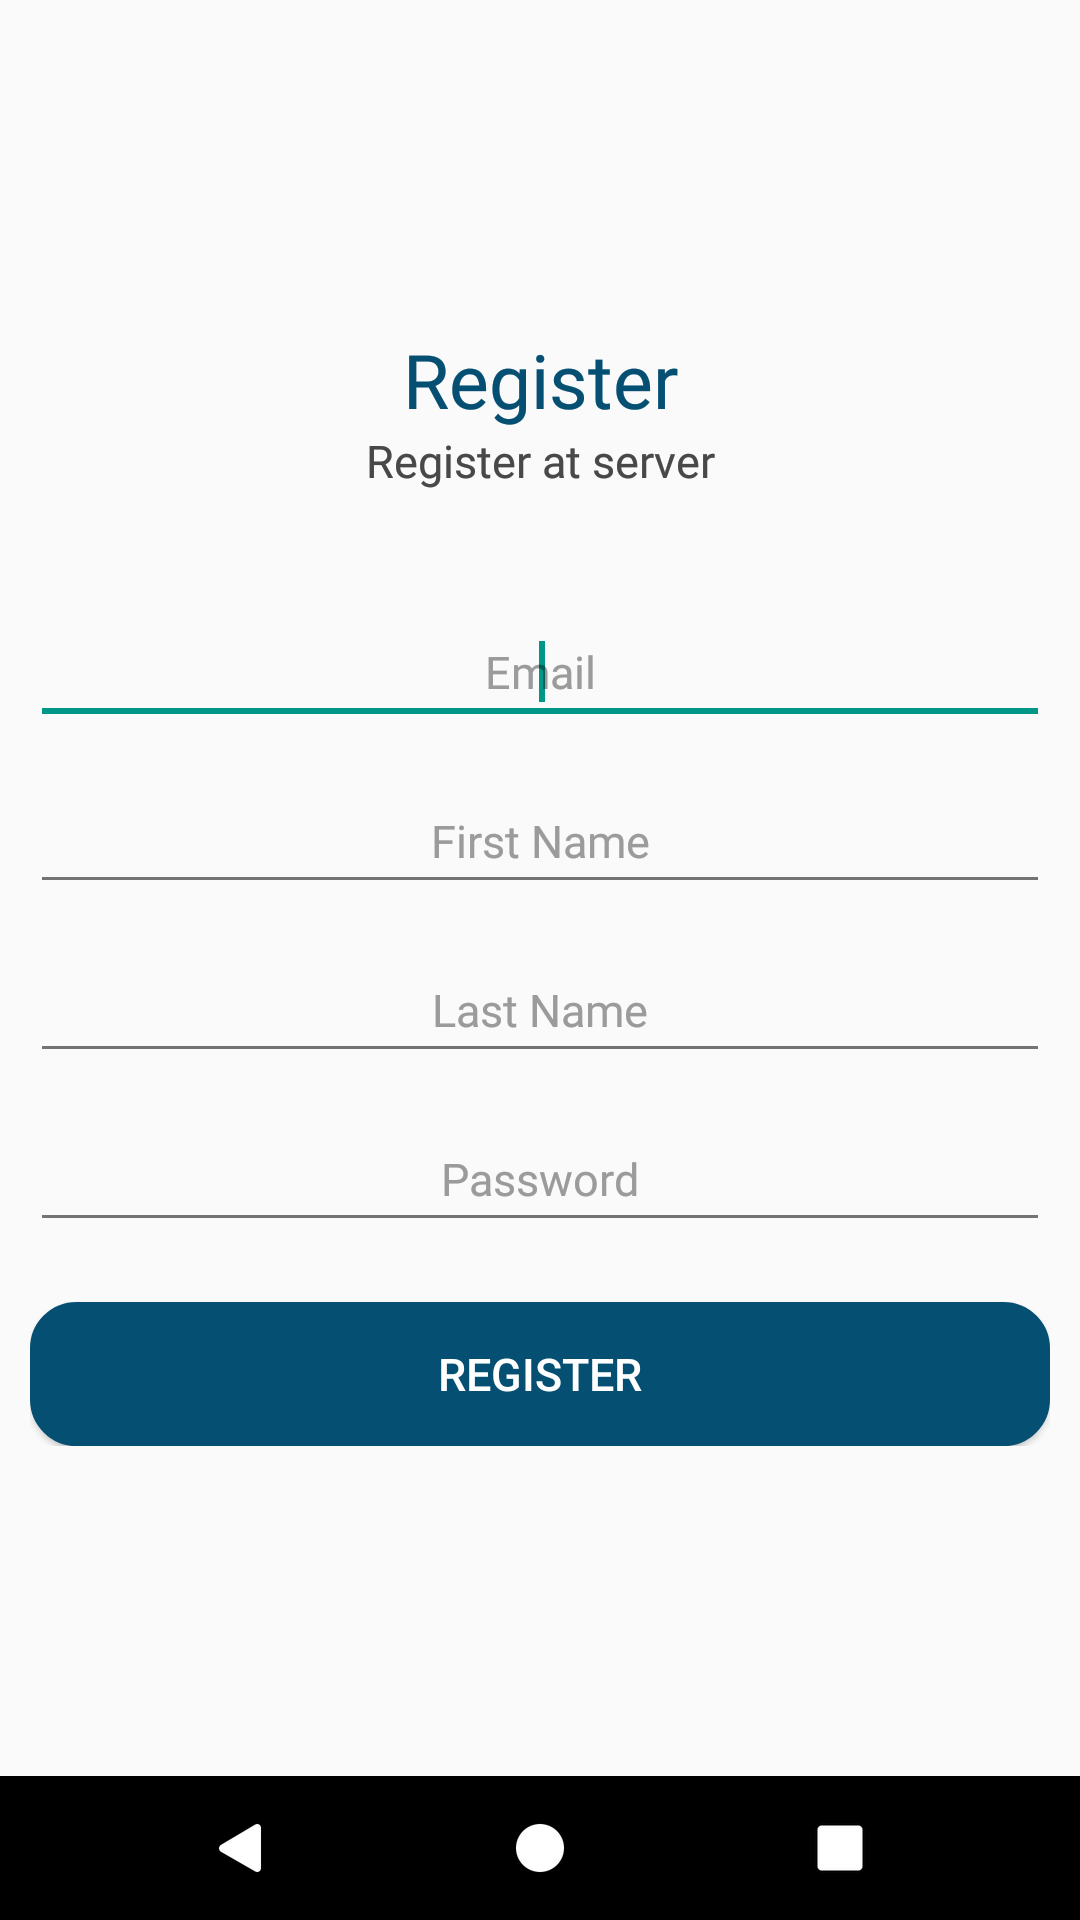
\includegraphics[width=\textwidth]{bilder/4_appRegister.png}
  \end{minipage}
  \caption{Login- und Registrierungs-Bildschirm der Voice Bank App}
  \label{fig:app-login}
\end{figure}

Hat sich ein Benutzer registriert, kann er sich unter Eingabe der Daten anmelden. Im Anschluss kann man Überweisungs-Vorlagen und die Anbindungen der Bankkonten verwalten. Für die App wird ebenfalls Firebase implementiert, um die vom Backend generierten Push-Nachrichten zu empfangen. Beim Registrieren eines Benutzers wird der Firebase Token in der Datenbank hinterlegt (\vgl Abbildung \ref{fig:datenbank-modell}). Dieser Token adressiert die Voice Bank App eines Benutzers für die Push-Nachrichten des Backends.

\subsection{Verwalten}
\label{subsec:app-verwalten}
Nachdem sich ein Benutzer angemeldet hat, erscheinen die Oberflächen für die Verwaltung der Vorlagen und Anbindungen. Abbildung \ref{fig:app-accounts} zeigt links die Liste der angebundenen Konten.

\begin{figure}[h]
  \centering
  \begin{minipage}[b]{0.45\textwidth}
    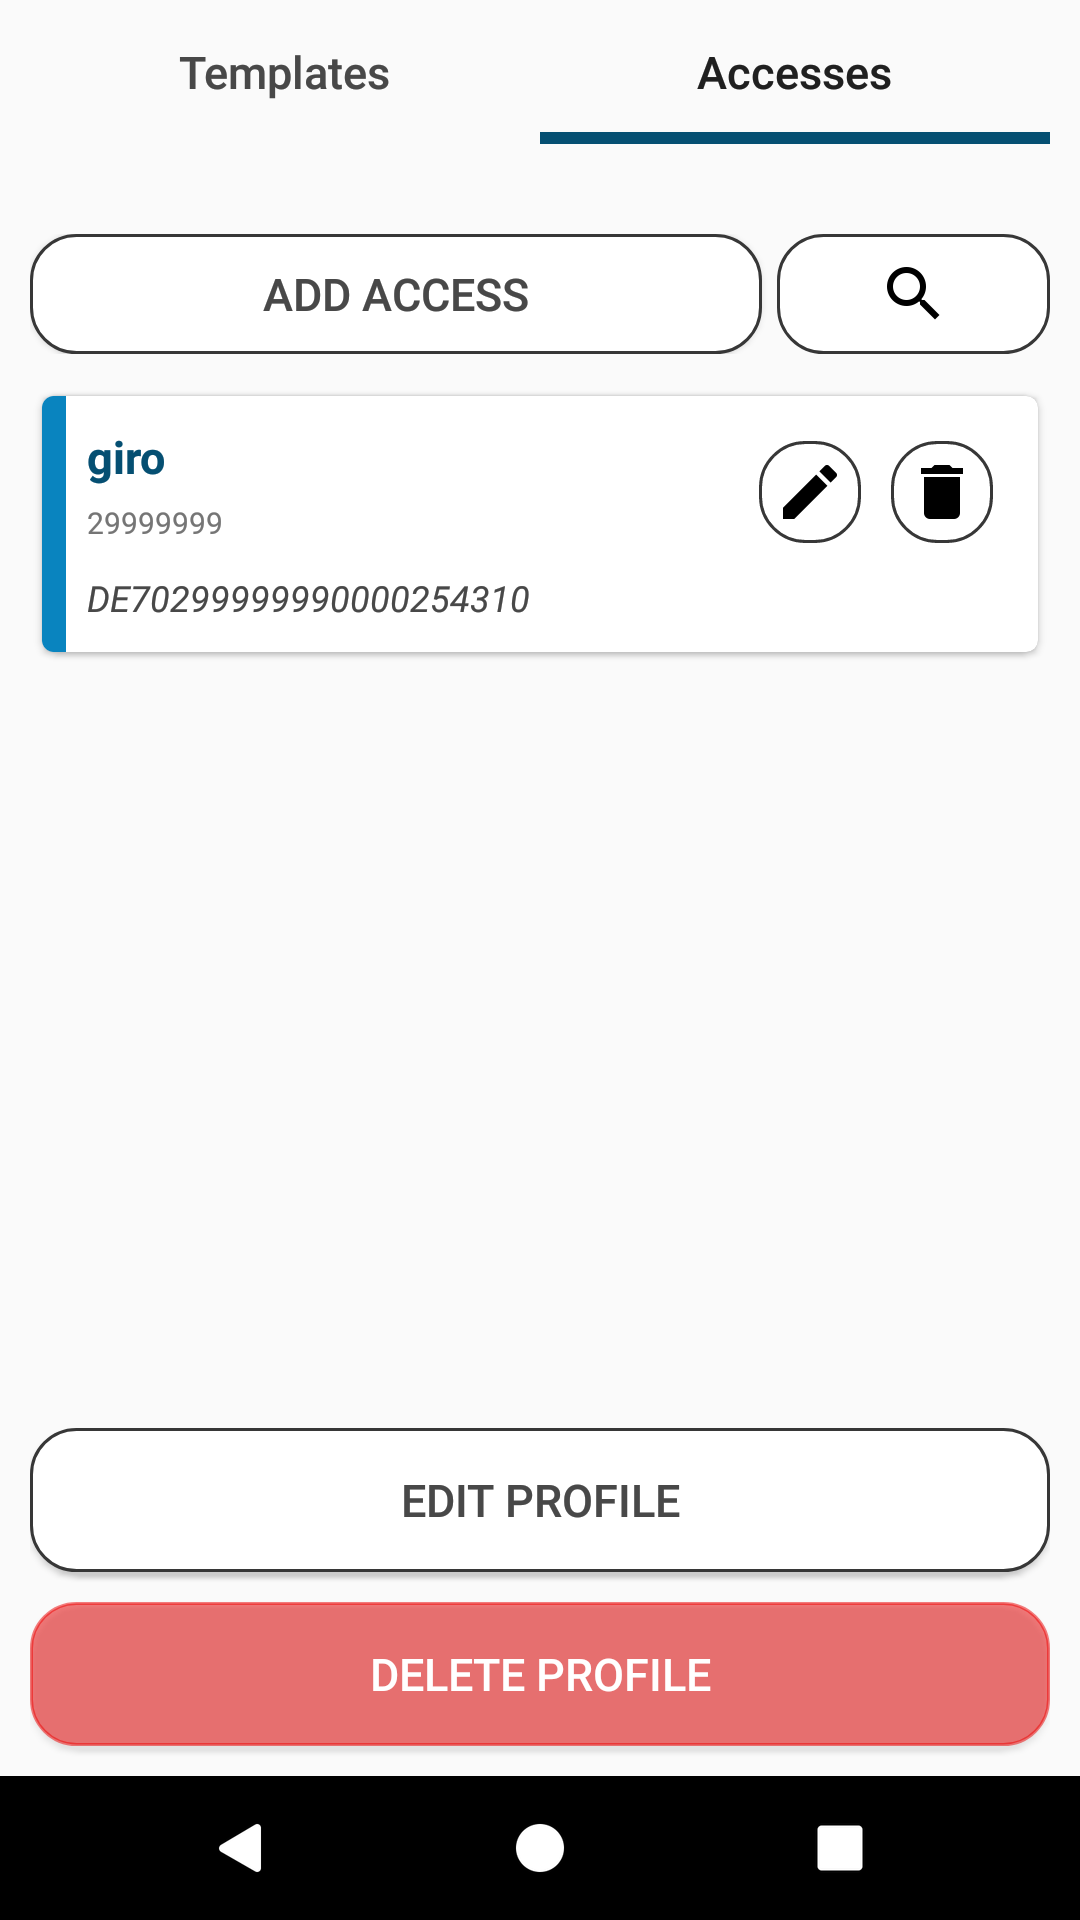
\includegraphics[width=\textwidth]{bilder/4_appAccounts.png}
  \end{minipage}
  \begin{minipage}[b]{0.45\textwidth}
    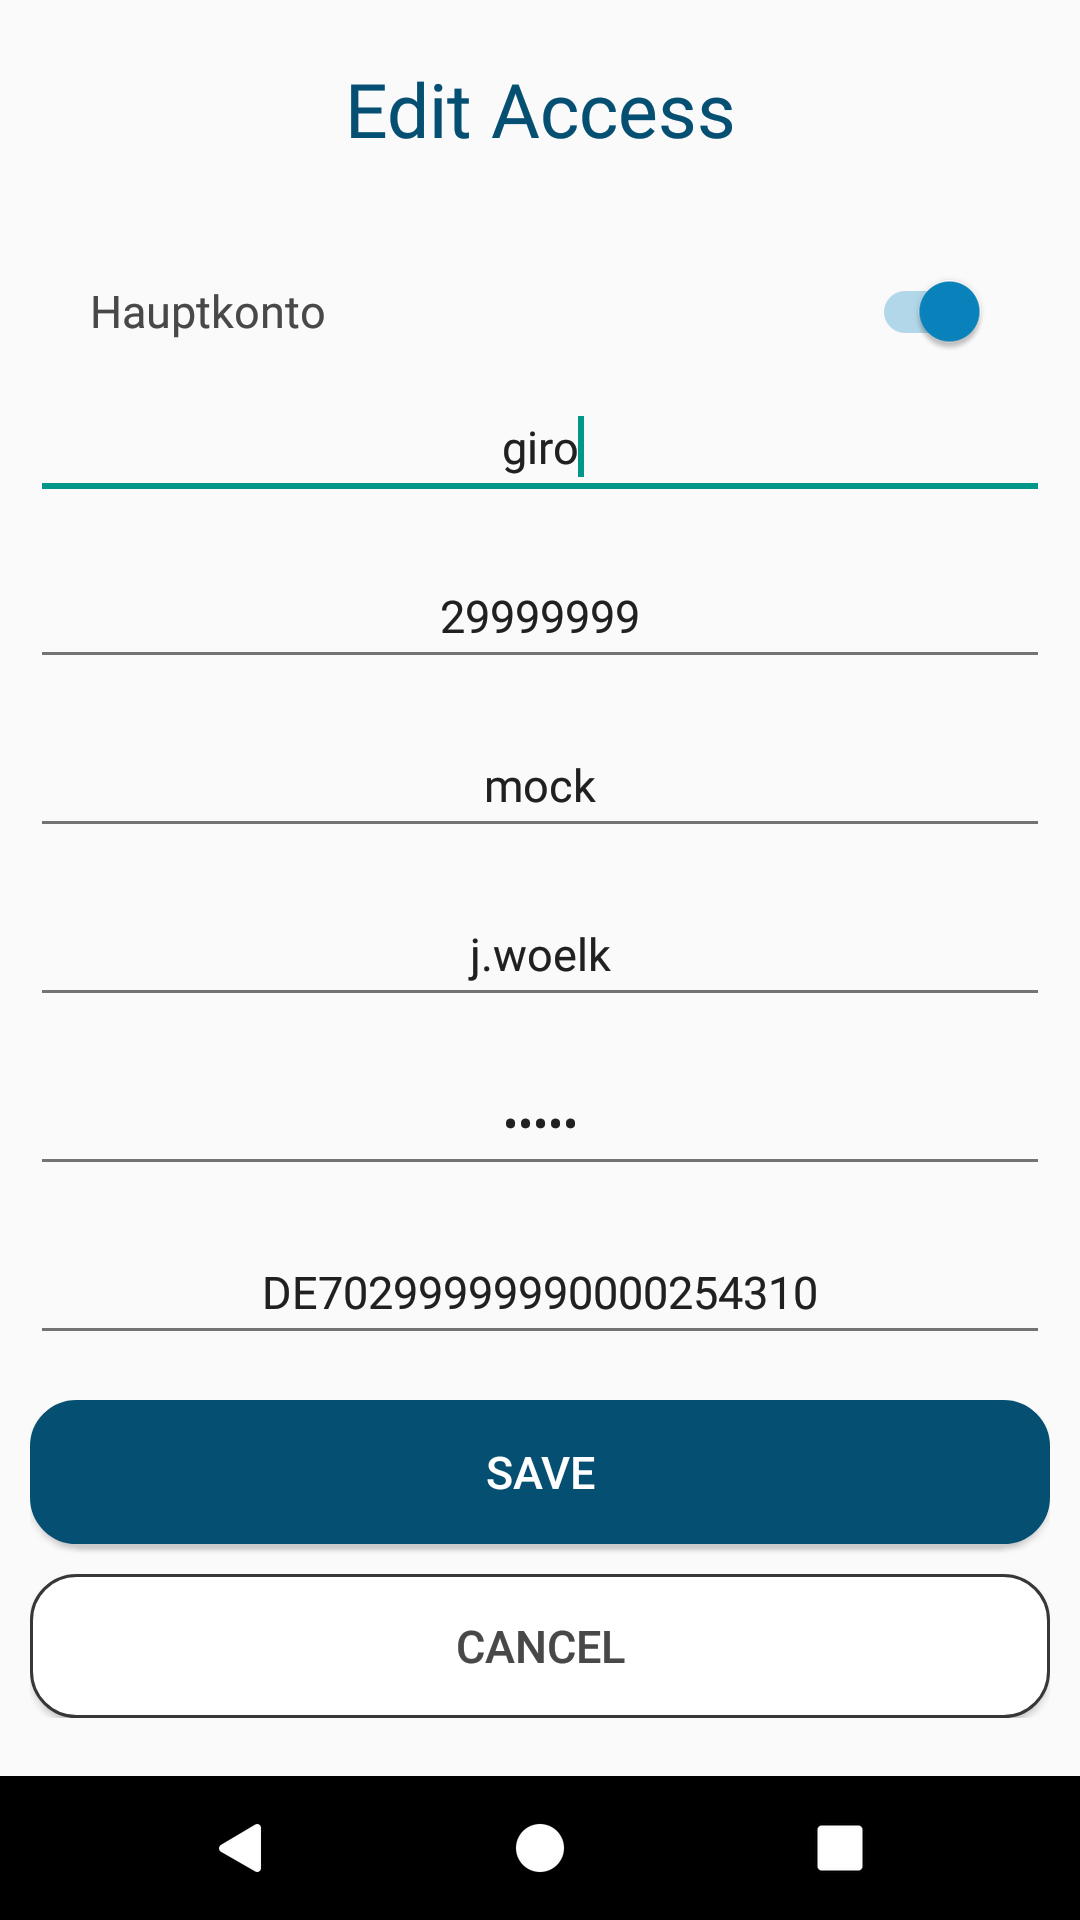
\includegraphics[width=\textwidth]{bilder/4_appMainAccount.png}
  \end{minipage}
  \caption{Bildschirm zur Anzeige und Bearbeitung der Bankkonten-Anbindungen}
  \label{fig:app-accounts}
\end{figure}

Jeder Datensatz wird in einem eigenen Reiter organisiert. Die Oberfläche für die Bearbeitung einer Anbindung wird rechts in Abbildung \ref{fig:app-accounts} dargestellt. Oben rechts ist dort auch die Schaltfläche zu sehen, mit der dieses Konto als „Hauptkonto“ gesetzt werden kann. In der Liste ist ein Hauptkonto durch eine blaue Markierung auf der linken Seite markiert. Falls viele Vorlagen erstellt oder Konten angebunden werden, kann das Suchfeld die Bedienung erleichtern. 

\subsection{Auf Push-Nachrichten reagieren}
\label{subsec:app-push}
Um die Aufforderung der Authentifzierung entgegen zu nehmen und die generierten \acp{TAN} zu empfangen wird Firebase verwendet. Durch Klicken auf die empfangene Push-Nachricht erscheint der Bildschirm mit der Aufforderung zur Bestätigung des Fingerabdruckes. Abbildung \ref{fig:app-auth} zeigt die empfangene Nachricht und den Bildschirm mit der Aufforderung. 

\begin{figure}[h]
  \centering
  \begin{minipage}[b]{0.45\textwidth}
    
\includegraphics[width=\textwidth]{bilder/4_appPushNachricht.png}
  \end{minipage}
  \begin{minipage}[b]{0.45\textwidth}
    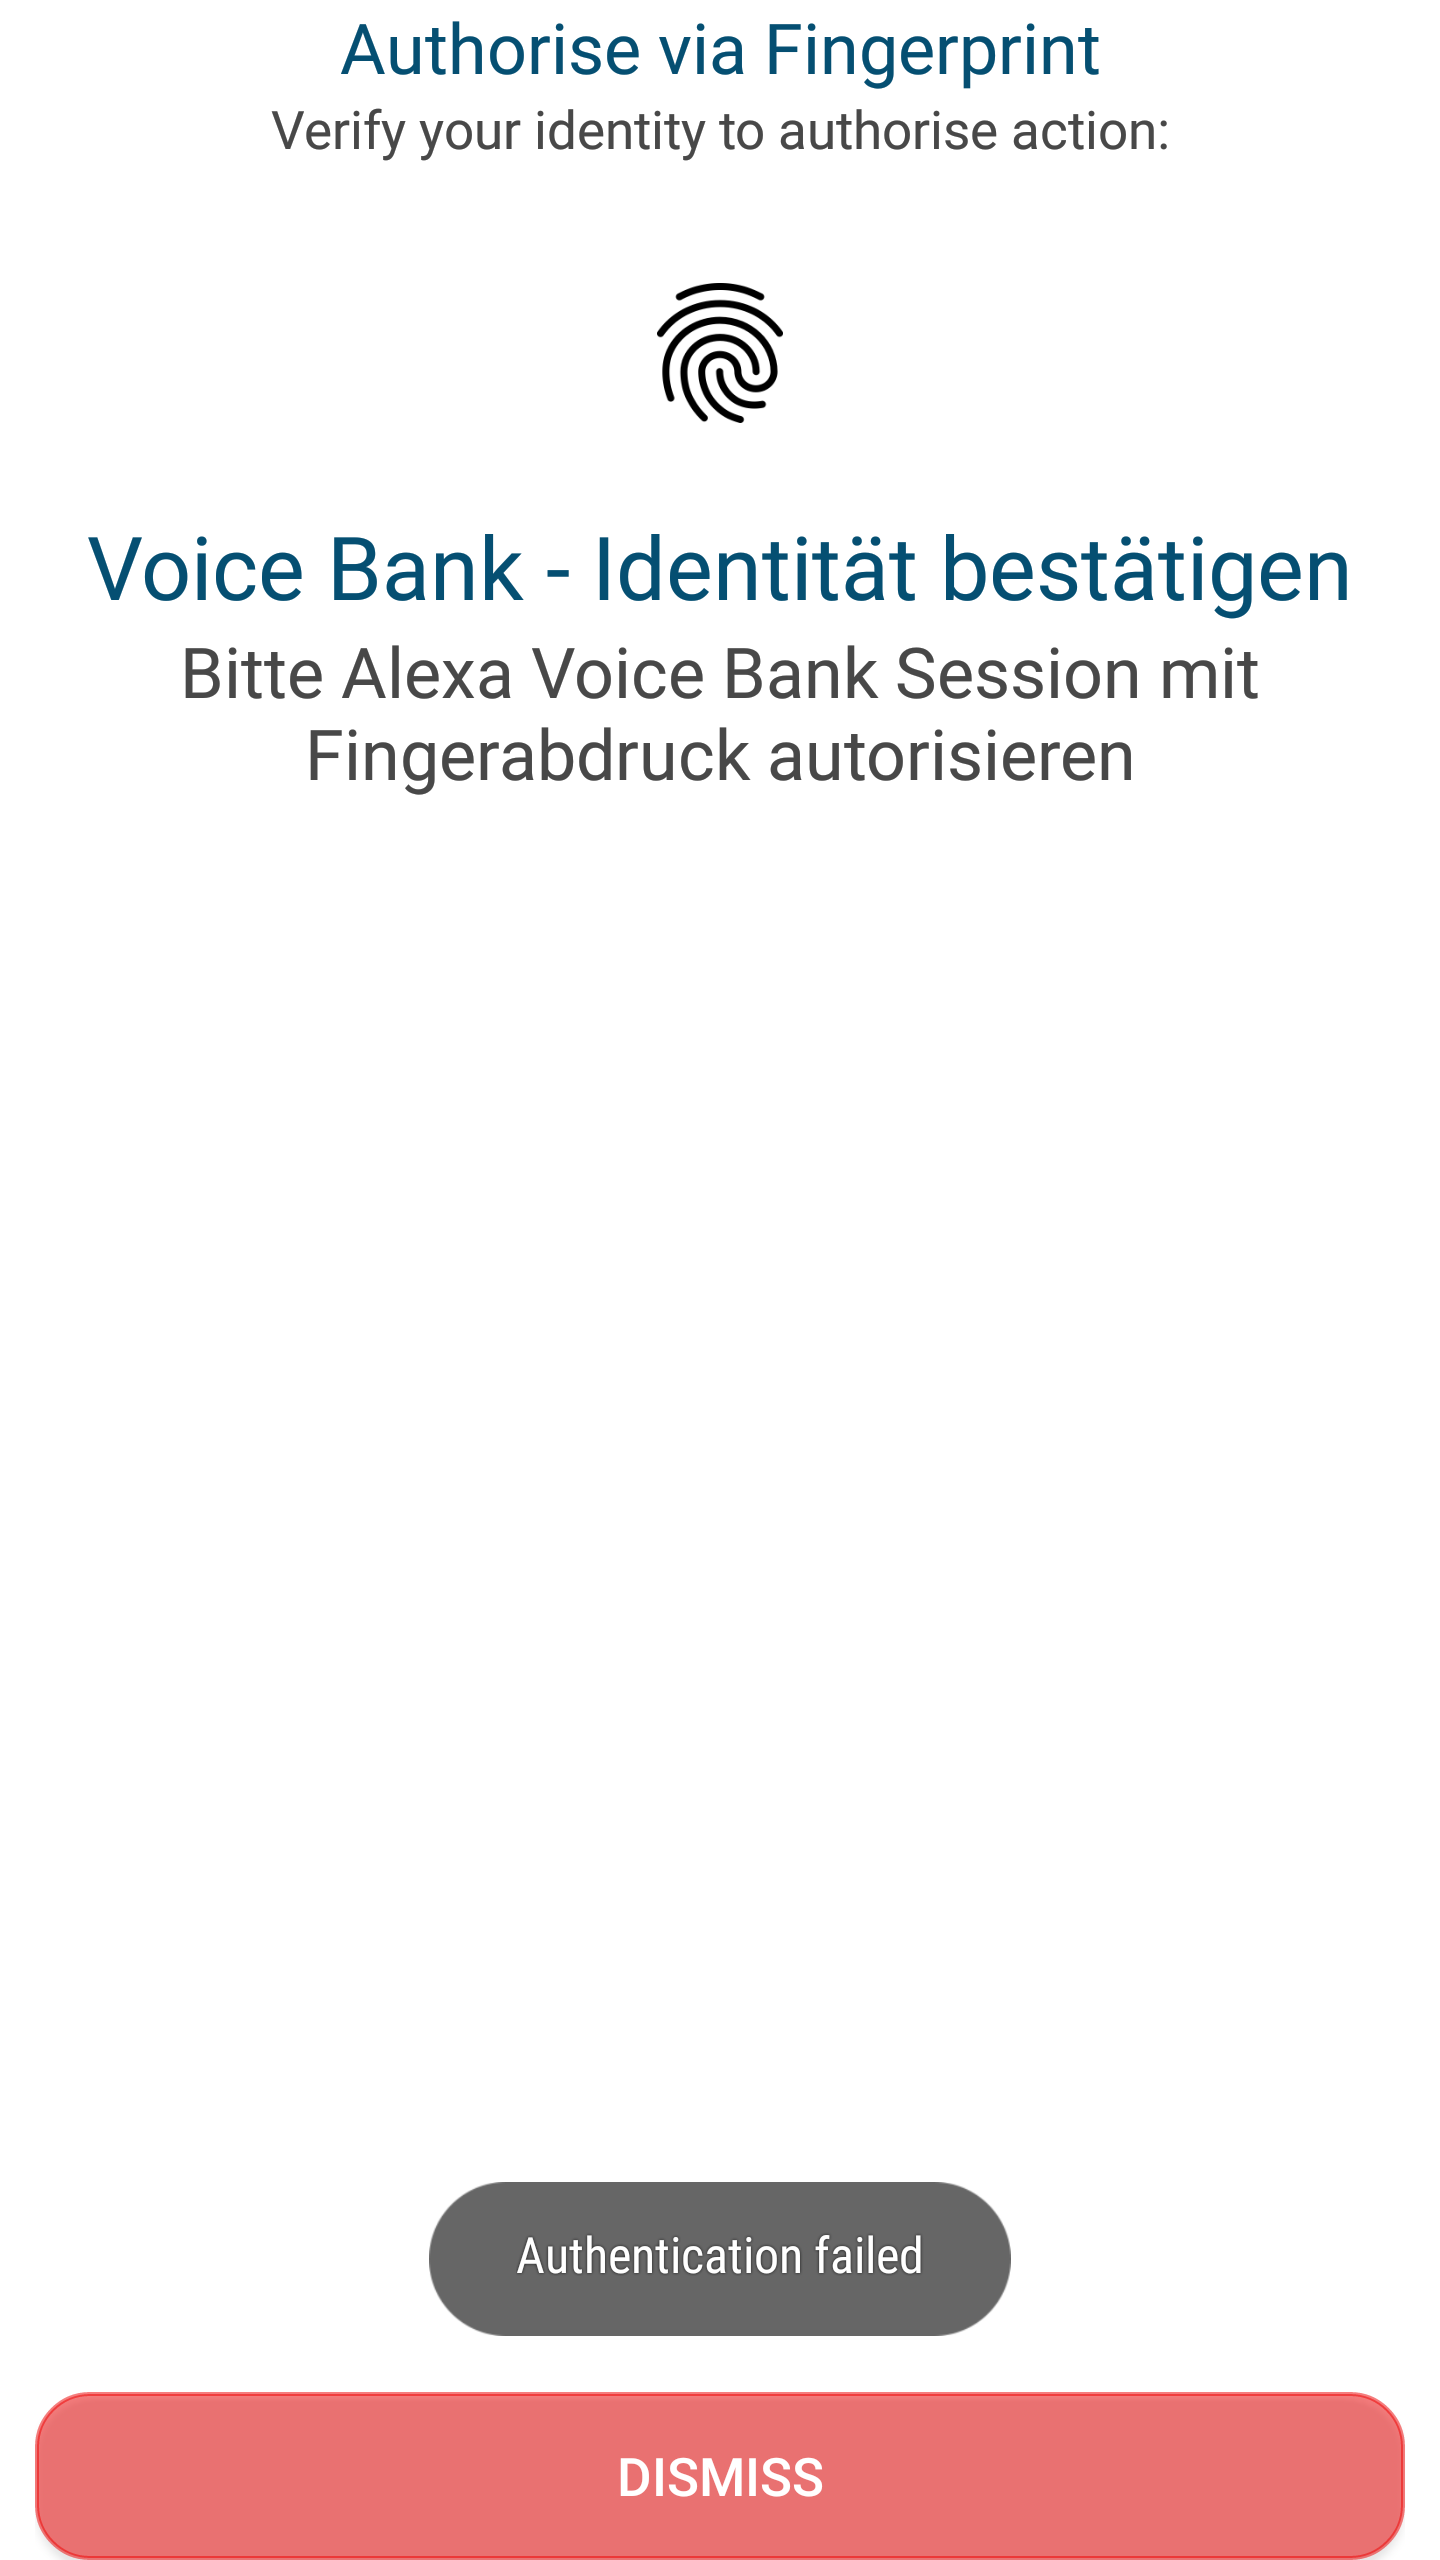
\includegraphics[width=\textwidth]{bilder/4_appAuthorise.png}
  \end{minipage}
  \caption{Bildschirm mit empfangener Push-Benachrichtigung und Aufforderung zur Authentifizierung}
  \label{fig:app-auth}
\end{figure}

Eine empfangene \ac{TAN} Nachricht dient lediglich der Anzeige der Nummer. Durch Klicken wird hier kein neuer Bildschirm geöffnet. Die folgenden Kapitel beschreiben die Implementierung des eigentlichen \ac{CUI}. Der Programmcode der Voice Bank App ist auf der beiliegenden CD unter \textit{„Quelltexte/finlexa\_android/“} zu finden.

\section{Skill-Server}
\label{sec:skill-server}
Aus Kapitel \ref{sec:alexa-voice-service} ist bekannt, dass der Skill-Server die Logik des \ac{CUI} abbildet. Die mit Hilfe des Interaction Model und der \ac{NLP} interpretierten Daten werden an den Skill-Server übermittelt. Hier müssen die entsprechenden Verknüpfungen mit dem Nutzungskontext stattfinden. Des Weiteren ist die Antwort zu generieren, die zurück an die Alexa Plattform geschickt wird. Dafür muss der Skill-Server ebenfalls eine \ac{REST}-Schnittstelle implementieren, die Alexa konsumieren kann. Der Server muss für die Alexa Plattform über das Internet zugänglich sein. Dabei gibt es mehrere Möglichkeiten für die Bereitstellung. Eine ist die Nutzung von \textit{Lambda}, einer sogenannten \textit{\ac{FaaS}}\footnote{FaaS ist ein Dienst, der von Cloud-Plattformen angeboten wird. Er ermöglicht die Entwicklung, Verwaltung und Bereitstellung von Applikationen ohne die sonst benötigte, komplexe Konfiguration einer Server Infrastruktur.}. Lambda ist Teil der \textit{\ac{AWS}} und erleichtert die Bereitstellung eines Skill-Servers in vielerlei Hinsicht. Ein Skill-Server muss verschiedene Voraussetzungen erfüllen, damit er von Alexa genutzt werden kann \cite{alexa-verify-request}.

\begin{itemize}
    \item Er muss über das Internet erreichbar sein
    \item Er muss gemäß der von Amazon definierten \ac{ASK}-Schnittstelle kommunizieren
    \item Er muss \ac{SSL}/\ac{TLS} unterstützen
    \item Er muss Anfragen auf Port 443 akzeptieren
    \item Er muss Anfragen von Alexa validieren
\end{itemize}

Fast alle der Anforderungen werden von Lambda \bzw \ac{AWS} übernommen. Zu erwähnen ist, dass \ac{AWS} nur ein Jahr lang kostenfrei benutzt werden kann\footnote{Mittlerweile kann AWS über das erste Jahr hinaus verwendet werden, wenn der Datenverkehr ein bestimmtes Kontingent nicht überschreitet}. Man ist jedoch nicht auf dessen Nutzung angewiesen. Für die Bereitstellung kann man jede Art von Web-Server verwenden, die diese Anforderungen erfüllt. Der Skill-Server wird in dieser Arbeit ebenfalls über einen eigenen Server bereitgestellt. Der Grund dafür ist in erster Linie, diese Art der Bereitstellung einmal selbst durchgeführt zu haben. Des Weiteren kann die Infrastruktur des Projektträgers ohne zusätzlichen Kostenaufwand verwendet werden. Der Prozess ist in Kapitel \ref{sec:deployment} näher beschrieben. Die Nutzung von Lamba wird hier nicht dokumentiert. Es gibt bereits zahlreiche Tutorials und Anleitungen, die sich im Detail damit beschäftigen \cite{aws-lambda}. Im nächsten Kapitel wird das \ac{ASK}-\textit{\ac{SDK}}\footnote{Ein \ac{SDK} ist typischerweise eine Ansammlung von Tools und bereits geschriebenem Programmcode, die bei der Entwicklung von Software-Anwendungen unterstützen.} vorgestellt. 

\subsection{Alexa Skills Kit SDK}
\label{subsec:skill-ask-sdk}
Ein gängiges Mittel für die Entwicklung eines Alexa Skills ist die Verwendung des \ac{ASK}-\ac{SDK} \cite{alexa-sdk}. Es stellt viele Dinge bereit und erleichtert damit den Entwicklungsprozess. Die folgenden Funktionalitäten sind \ua Teil des \ac{SDK}.

\begin{itemize}
    \item \textit{Request handling}: Es unterstützt bei der Verarbeitung der eingegangenen Anfragen von Alexa. \ac{JSON} Daten werden bereits geparsed, das heißt für die weitere Verarbeitung als nutzbares Objekt angeboten. Für definierte Intents kann man auf einfache Weise die Funktionen mit der entsprechenden Logik adressieren.
    
    \item \textit{Session handling}: Da \ac{REST} im Allgemeinen zustandslos ist, erfolgt die Interaktion mit einem Skill in sogenannten Sessions. Es handelt sich dabei um ein Objekt, welches relevante Daten im Zuge einer Konversation speichern kann. In der Regel ist eine Session vom Start des Skills bis zu dessen Beendigung aktiv. Das \ac{SDK} unterstützt beim Handhaben des Session-Objektes. Konkret vereinfacht es die Erstellung und Bearbeitung. 
    
    \item \textit{State handling}: Ein Skill kann verschiedene Zustände einnehmen. Diese können frei vom Entwickler definiert werden. Auch hierbei unterstützt das \ac{SDK} bei der Handhabung dieser Stati. 
    
    \item \textit{Response building}: Die \ac{ASK} Schnittstelle arbeitet unter Verwendung einer definierten \ac{JSON} Syntax. Sowohl Anfragen von Alexa, als auch die Antworten müssen diesem Schema entsprechen \cite{alexa-response-request-format}. Unter Verwendung des \ac{SDK} müssen lediglich die Antworten selbst generiert werden. Es erstellt im Anschluss die notwendigen Strukturen für die Antwort.
\end{itemize}

Auch wenn es sichtlich viele Vorteile bietet, ist die Nutzung des \ac{SDK} auch mit einer gewissen Einschränkung verbunden. Bei der Entwicklung muss man den vorgegebenen Paradigmen folgen. Gerade beim Verarbeiten der eingegangenen Anfragen hat man als Entwickler erst spät Einfluss auf den weiteren Weg der Anfrage. Der Einstiegspunkt sind die für die Intents adressierten Funktionen, auch Handler genannt. Da das Bewusstsein für den Kontext eine der Anforderungen an das \ac{CUI} ist (\vgl Kapitel \ref{sec:conversational-user-interface}), soll der Skill-Server auch dementsprechend kontextbasiert agieren. Das erfordert die Anfrage auszuwerten und selbst zu entscheiden, welche Handler für diesen Kontext in Frage kommen. Eine weitere Einschränkung gilt der Auswertung der Slots, was gerade für den Banking Skill ein Problem darstellt. Für ein besseres Verständnis wird dies anhand eines Beispiels erklärt.\\
Hierfür werden die Intents „Transaktion via Vorlage“ und „Sparziel“ verwendet. Beide benötigen einen „Name“ Slot für die Verarbeitung. Für die Transaktion ist das der Name der verwendeten Überweisungsvorlage, während das Sparziel den Namen des Themas benötigt, für das gespart werden soll. Aus Kapitel \ref{sec:alexa-voice-service} ist bekannt, dass sämtliche Formulierungen für Alexa vorgegeben werden müssen. Das schließt auch die Formulierungen ein, die Benutzer im Fall von fehlenden Slots verwenden. Auch wenn das Interaction Model in Kapitel \ref{sec:interaction-model} beschrieben ist, wird hier für das Verständnis eine Erklärung benötigt. Eine Utterance für das Beispiel der Transaktion wäre:\\\\
Transaktion \textit{Überweise \{Betrag\} an \{Name\}}
\\\\
An erster Stelle steht der Intent, der über die angegebene Formulierung angesprochen wird. Danach ist die eigentliche Formulierung mit ihren Slots, hier „Betrag“ und Name“, gegeben. Die Möglichkeit besteht, dass ein Nutzer lediglich den Betrag nennt. Der Skill sollte dann auf den fehlenden Namen aufmerksam machen und \zB das Folgende ausgeben:
\begin{center}
   \textcolor{mybluelight}{Alexa: „An wen möchtest du überweisen?“}
\end{center}
Gemäß den User Tests aus Kapitel \ref{sec:prototyping}, hat jeder Benutzer diese Frage alleine mit dem entsprechenden Namen beantwortet. Die Utterance hierfür sieht also folgendermaßen aus:\\\\
Transaktion\textit{\{Name\}}\\\\
Denkt man nun an alle Intents, die einen derartigen Slot beinhalten, wie \zB der Sparziel Intent oder der Intent für Informationen zu Umsatzdaten, sehen deren Utterances für diesen Fall identisch aus.\\\\
    Transaktion \textit{\{Name\}}\\
    Sparziel \textit{\{Name\}}\\
    UmsatzInformation \textit{\{Name\}}\\\\
Alexa kann Intents lediglich anhand der im Interaction Model hinterlegten Formulierungen unterscheiden. An dieser Stelle gibt es also ein Problem. Nennt ein Benutzer einen Namen, kann Alexa nicht differenzieren, welcher der Intents angesprochen werden muss. Größtenteils wird der erste angesprochen, der mit der Eingabe übereinstimmt. In diesem Fall ist das die Transaktion. Aus den genannten Gründen wird das \ac{SDK} nicht in dieser Arbeit verwendet\footnote{Im Verlauf dieser Arbeit wurde das \ac{SDK} von Amazon erweitert. Die beschriebenen Einschränkungen können dadurch gelöst werden. Da nach einer Evaluierung der Ansatz aus Kapitel \ref{subsec:skill-architektur} dennoch als flexibler erachtet wird, wurde dieser weiter verfolgt.}. Kapitel \ref{subsec:skill-architektur} beschreibt die Entwicklung einer Architektur, mit deren Hilfe der Skill-Server implementiert werden kann.

\subsection{Architektur}
\label{subsec:skill-architektur}
Aufgrund der in Kapitel \ref{subsec:skill-ask-sdk} genannten Einschränkungen des \ac{SDK}, wird eine Architektur für den Skill-Server entwickelt. Diese soll in erster Linie die beschriebenen Probleme lösen. Abbildung \ref{fig:skill-architektur-komponenten} zeigt das Ergebnis in Form einer Komponentenübersicht.

\begin{figure}[!htb]
    \centering
    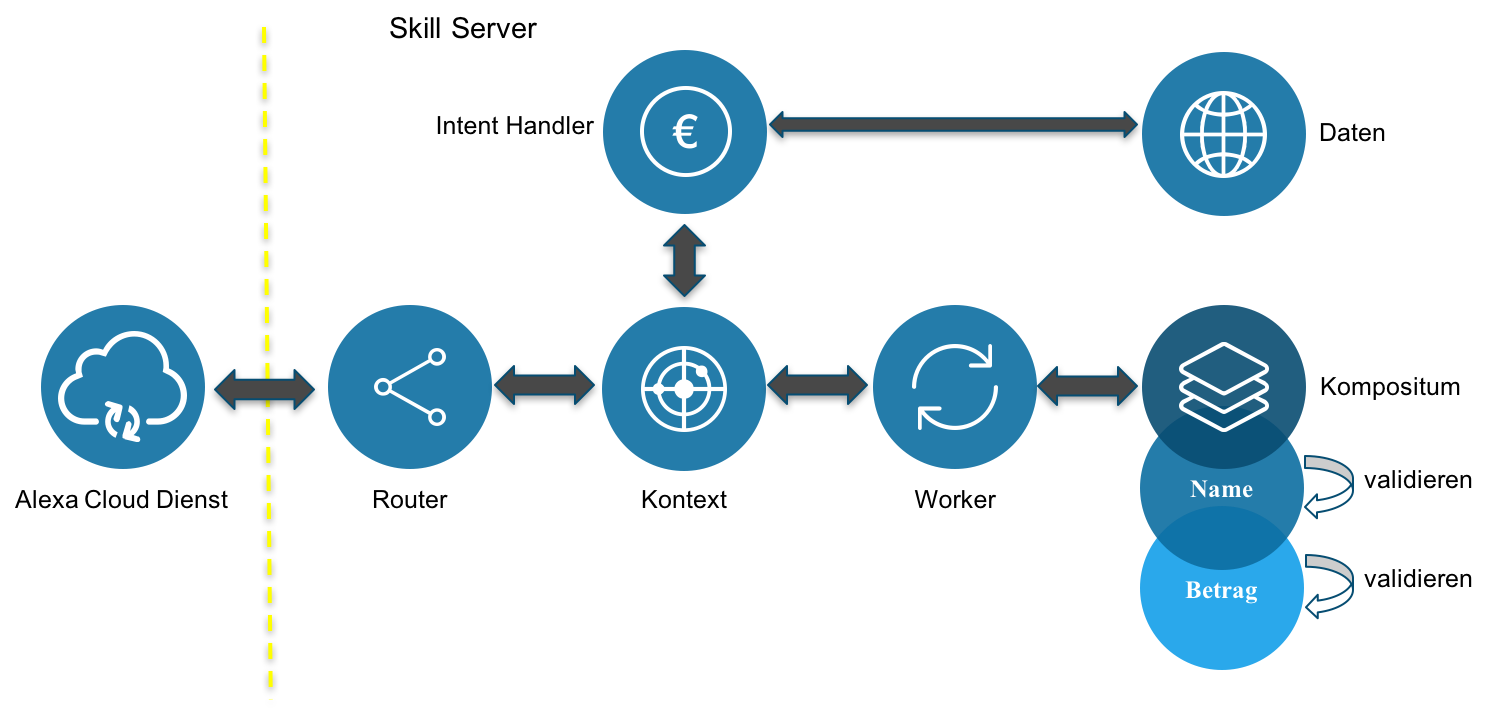
\includegraphics[width=1.0\textwidth]{bilder/4_skillArchitektur.png}
    \caption{Komponentenübersicht der Architektur}
    \label{fig:skill-architektur-komponenten}
\end{figure}

Alexa sendet eine Anfrage an den Skill-Server. Entsprechend der Daten baut dieser den Kontext auf. Der Kontext erstellt auf Basis der für den Intent benötigten Slots und deren Werte eine Worker Instanz. Der Worker hält ein \textit{Kompositum}\footnote{Ein Entwurfsmuster aus der Software Entwicklung \cite{freeman-headfirst-patterns}} mit diesen Slots, die nun sequentiell validiert werden. Falls Slots fehlen oder eingegebene Werte vom Benutzer bestätigt werden müssen, wird die Antwort vom Worker generiert und über den Kontext zurück an die Alexa Plattform gesendet. Bei erfolgreicher Validierung gibt der Worker keine Antwort an den Kontext zurück. Die Parameter werden dann an den Intent Handler übermittelt, worauf dieser ausgeführt wird. Die entsprechende Logik wird durchlaufen und \ggf werden relevante Daten über weitere Dienste beschafft. Im Anschluss generiert er die Antwort und gibt sie dem Kontext zurück. Dieser überträgt die Antwort wiederum an die Alexa Plattform.\\
Der aktuelle Kontext besteht also aus dem Intent und dem Kompositum mit den entsprechenden Slots. Aus Kapitel \ref{subsec:skill-ask-sdk} ist das Alexa Session-Objekt bereits bekannt. Bevor der Skill-Server eine Antwort zurück zur Alexa Plattform sendet, wird dieses mit dem aktuellen Kontext beschrieben. Bei der nächsten Anfrage, kann man auf das gleiche Objekt zurückgreifen. Entsprechend dessen und der neuen Daten vom Benutzer wird ein neuer Kontext aufgebaut, die Slots mit \ggf neuen Werten validiert und der Intent Handler ausgeführt. Geht man zum Problem der Slot Validierung aus Kapitel \ref{subsec:skill-ask-sdk} zurück, bietet dieses Vorgehen eine mögliche Lösung. Anstatt jedem der Intents eine Formulierung mit dem Slot „Name“ zuzuweisen, gibt es einen eigenen Intent für diesen Slot. Im Interaction Model sieht das folgendermaßen aus: \\\\
Transaktion \textit{Überweise \{Betrag\} an \{Name\}}\\
Name \textit{\{Name\}}\\
Betrag \textit{\{Betrag\}}\\

Nennt ein Benutzer lediglich den fehlenden Namen, gibt es nur noch einen Intent, der angesprochen werden kann. Diese speziellen Intents werden im Folgenden als \textit{Atomic Intents} bezeichnet. Der Wert des Slots kann nun vom Skill-Server kontextbezogen verarbeitet und an den richtigen Intent Handler adressiert werden. Im Falle einer Transaktion wird der Atomic Intent „Name“ als Name der verwendeten Überweisungsvorlage gehandhabt. Man kann also sagen, dass das Kompositum in Abbildung \ref{fig:skill-architektur-komponenten} aus Atomic Intents zusammengesetzt wird. Kapitel \ref{subsec:skill-implementierung} beschreibt die Umsetzung der hier beschriebenen Architektur. 

\subsection{Implementierung}
\label{subsec:skill-implementierung}
Im Folgenden wird der Skill-Server auf Basis der in Kapitel \ref{subsec:skill-architektur} beschriebenen Architektur umgesetzt. Wie das Backend, ist der Skill-Server mit Node.js, Express und TypeScript implementiert. Die Gründe dafür sind in Kapitel \ref{backend-plattform} genannt. Node.js ist für die Skill Entwicklung die am weitesten verbreitete  Plattform. Erwähnenswert sind außerdem zwei weitere \ac{npm} Module, die hier verwendet werden. 

\textbf{Bespoken Tools}\\
Dabei handelt es sich um einen Verbund an Tools, welche die Entwicklung von Alexa und Google \ac{VUI} Anwendungen unterstützen \cite{bespoken}. Unabhängig davon, ob man den Skill über \ac{AWS} oder einem eigenen Web Server bereitstellt, nimmt der Prozess der Auslieferung (Deployment) einige Minuten in Anspruch. Um Zeit zu sparen ist es wesentlich angenehmer lokal zu entwickeln und zu testen. Da ein Skill-Server über das Internet für Alexa erreichbar sein muss, ist das normalerweise nicht möglich. Mit Hilfe der Bespoken Tools kann genau das erreicht werden, indem ein Proxy Dienst eingerichtet wird. Die Konfiguration dauert nur wenige Minuten und wird mit Hilfe der Kommandozeile durchgeführt. Das Tool gibt eine \textit{\ac{URL}} aus. Diese wird auf der Alexa Plattform als Adresse des Skill-Servers eingetragen. Startet man nun den Proxy und Skill-Server lokal, kann Alexa diese über den Proxy Dienst erreichen und nutzen, zu sehen in  Abbildung \ref{fig:bst-proxy} \cite{bespoken}.

\begin{figure}[!htb]
    \centering
    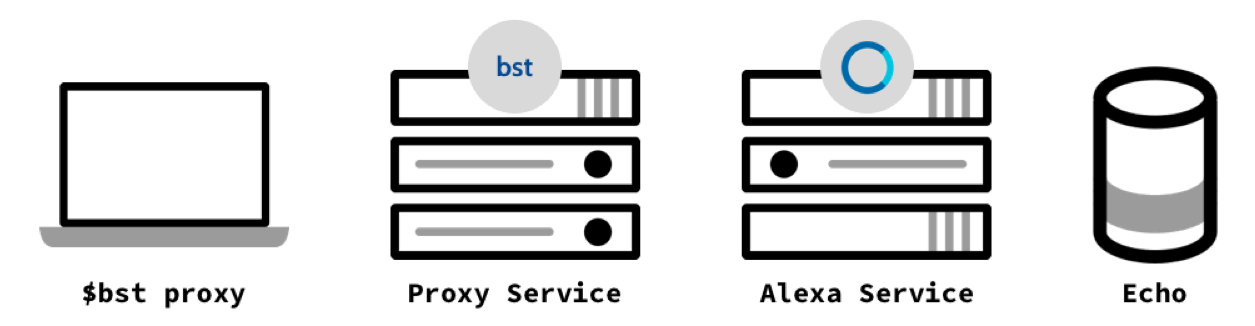
\includegraphics[width=0.8\textwidth]{bilder/4_bstProxy.png}
    \caption{Bespoken Tools Proxy Dienst}
    \label{fig:bst-proxy}
\end{figure}

Der Proxy ist nur eine der Anwendungen von Bespoken. Auf Weitere wird im Zuge dieser Arbeit nicht eingegangen, da lediglich die hier beschriebene verwendet wird.

\textbf{Alexa Verifier Middleware}\\
Mit Hilfe dieses Moduls können Anfragen von Alexa validiert werden \cite{alexa-verify-request}. Somit werden einige der in Kapitel \ref{sec:skill-server} genannten Voraussetzung eines Skill-Servers erfüllt. Mit Hilfe von Express kann dieses Modul über zwei Zeilen Quelltext eingesetzt werden. 

\textbf{Umsetzung}\\
Im Anschluss folgt die Umsetzung der in Kapitel \ref{subsec:skill-architektur} beschriebenen Architektur. Angefangen mit einer groben Übersicht in Abbildung \ref{fig:skill-komponenten}, werden die hellblau hinterlegten Komponenten im weiteren Verlauf näher beschrieben. Die Übersicht aus Kapitel \ref{subsec:skill-architektur} unterscheidet sich von der hier gezeigten Abbildung und stellt lediglich den Anfangsgedanken der Implementierung dar. Die Unterschiede in Abbildung \ref{fig:skill-komponenten} sind auf die Gegebenheiten der verwendeten Plattform und auf die Weiterentwicklung dieses Gedankens zurückzuführen.

\begin{figure}[!htb]
    \centering
    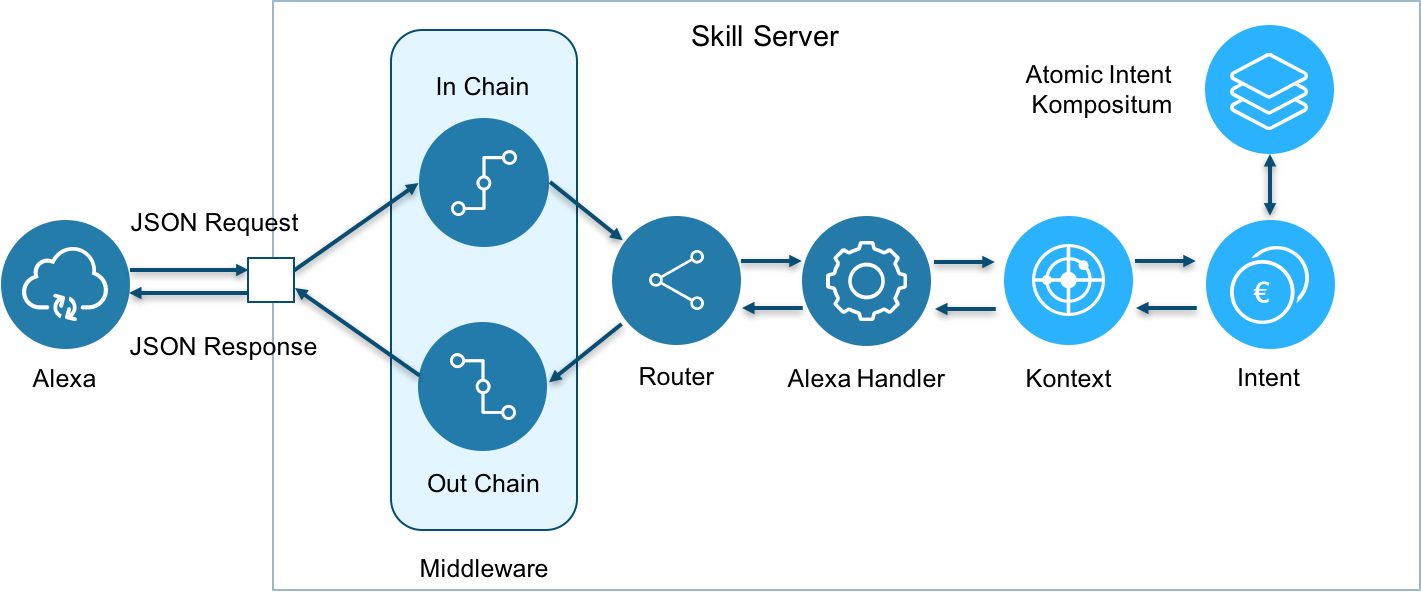
\includegraphics[width=1.0\textwidth]{bilder/4_skillKomponenten.png}
    \caption{Komponentenübersicht des Skill-Servers}
    \label{fig:skill-komponenten}
\end{figure}

Alexa sendet eine \ac{JSON} Anfrage (Request) an den Endpunkt des Servers. Die Anfrage passiert zunächst die Middleware. Diese besteht zum einen aus der „In Chain“, die \ua die beschriebene Alexa Verifier Middleware enthält. Zum anderen aus der „Out Chain“, welche die Antwort (Response) des Skills lediglich weitergibt. Der Router leitet die Request entsprechend ihres Ziels zur registrierten Handler Funktion. Hier gibt es nur eine Route, die den Alexa Handler adressiert. Dieser erstellt mit Hilfe der Daten aus der Request den Kontext. Die Daten umfassen \ua das Session-Objekt und die analysierten Informationen der Alexa \ac{NLP} mit dem vom Benutzer angesprochenen Intent, enthaltenen Slots und deren Werte. Ist der Kontext erstellt, wird dieser vom Alexa Handler ausgeführt.\\
Über den Kontext wird ein Intent erzeugt. Dieser baut wiederum sein Kompositum aus Atomic Intents auf, welches mit den übergebenen Slot Werten validiert wird. Außerdem hält der Intent die Logik. Nach der Validierung des Kompositums entscheidet diese, ob Daten vom Multibanking-Mock beschafft werden müssen und welche Antwort generiert wird. Die Antwort wird über den Kontext an den Handler zurückgegeben. Der Alexa Handler bettet die Phrasen in die \ac{JSON} Syntax ein, die Alexa verstehen kann. Dabei wird auch das Session-Objekt mit dem aktuellen Kontext beschrieben. Das \ac{JSON} Response Objekt wird dann über die Out Chain der Middleware zurück an Alexa gesendet und vom Echo ausgegeben. Im Folgenden werden mit Hilfe von Klassen- und Sequenzdiagrammen die Abhängigkeiten und Prozesse der in Abbildung \ref{fig:skill-komponenten} hellblau hinterlegten Komponenten näher betrachtet. Für einen besseren Überblick wird die Architektur dabei in kleinere Ausschnitte zerlegt.\\
Die Namen der Klassen, Funktionen und Typen in den Diagrammen sind den englischen Begriffen aus der Implementierung nachempfunden. Abbildung \ref{fig:skill-klassen-kontext} zeigt ein Klassendiagramm, dass die Kontext und Intent Komponenten aus Abbildung \ref{fig:skill-komponenten} näher beschreibt. 

\begin{figure}[!htb]
    \centering
    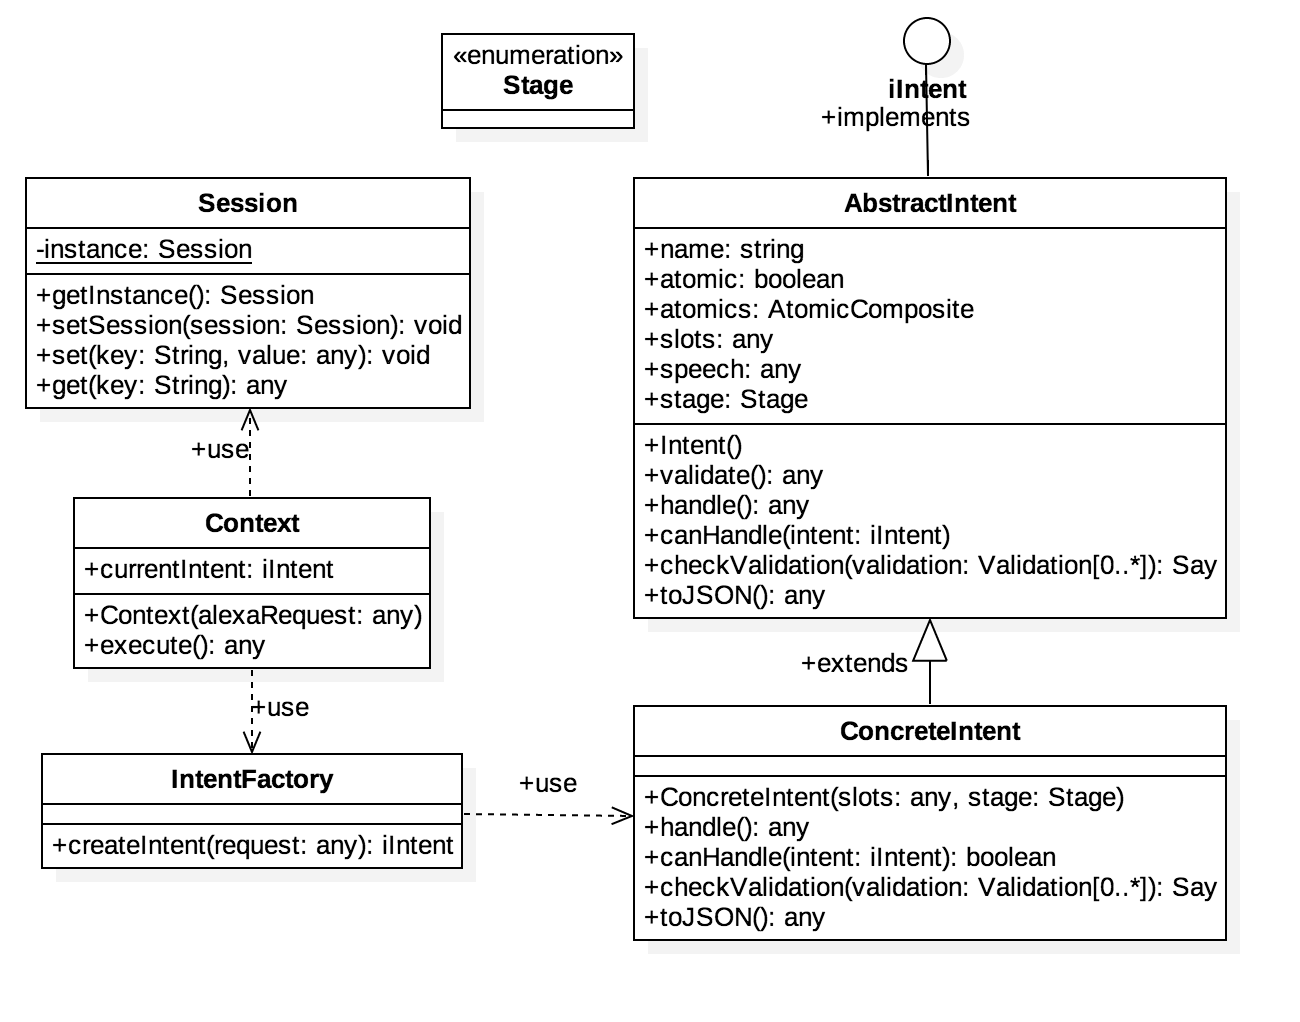
\includegraphics[width=1.0\textwidth]{bilder/4_klassenContext.png}
    \caption{Vereinfachtes Klassendiagramm von Kontext und Intent}
    \label{fig:skill-klassen-kontext}
\end{figure}

Die Kontext Klasse hat einen Konstruktur und die „execute“ Funktion. Im Konstruktor wird zunächst das Session-Objekt der Alexa Request ausgewertet. Die Session Klasse hilft hier beim Auslesen und Modifizieren dieses Objektes. Ist dort noch kein Intent aus vorherigen Interaktionen vorhanden, wird über die Factory ein neuer erstellt und als „currentIntent“ gesetzt. Die Factory ist, wie das Kompositum, ein Entwurfsmuster aus der Softwareentwicklung \cite{freeman-headfirst-patterns}. Sie ist für die Instanziierung eines konkreten Intents zuständig. Nachdem der Kontext erstellt ist, führt der Alexa Handler die execute Funktion aus, die wiederum die „handle“ Funktion des konkreten Intents ausführt. Der Intent gibt entsprechend seiner Logik eine Antwort über den Kontext zurück an den Alexa Handler. Das Sequenzdiagramm aus Abbildung veranschaulicht diesen Prozess.

\begin{figure}[!htb]
    \centering
    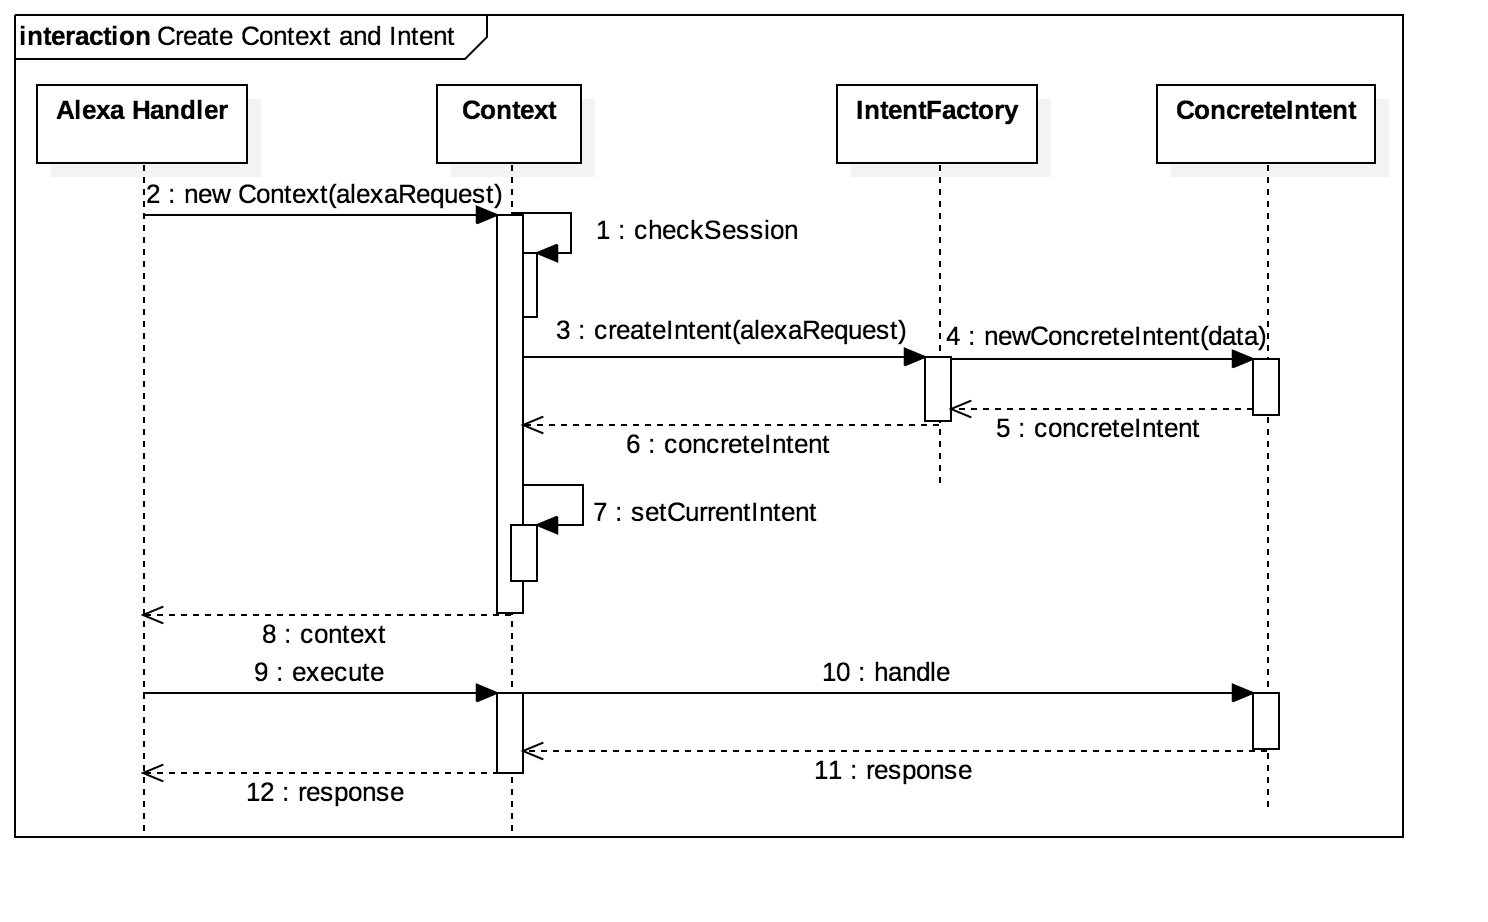
\includegraphics[width=1.0\textwidth]{bilder/4_skillSequenzKontextIntent.png}
    \caption{Sequenzdiagramm Instanziierung von Kontext und Intent}
    \label{fig:skill-sequenz-kontext}
\end{figure}

Im Folgenden wird das Zusammenspiel der Intent und Kompositum Komponente aus Abbildung \ref{fig:skill-komponenten} erläutert. Abbildung \ref{fig:skill-klassen-intent} stellt das entsprechende Klassendiagramm dar.\newpage

\begin{figure}[!htb]
    \centering
    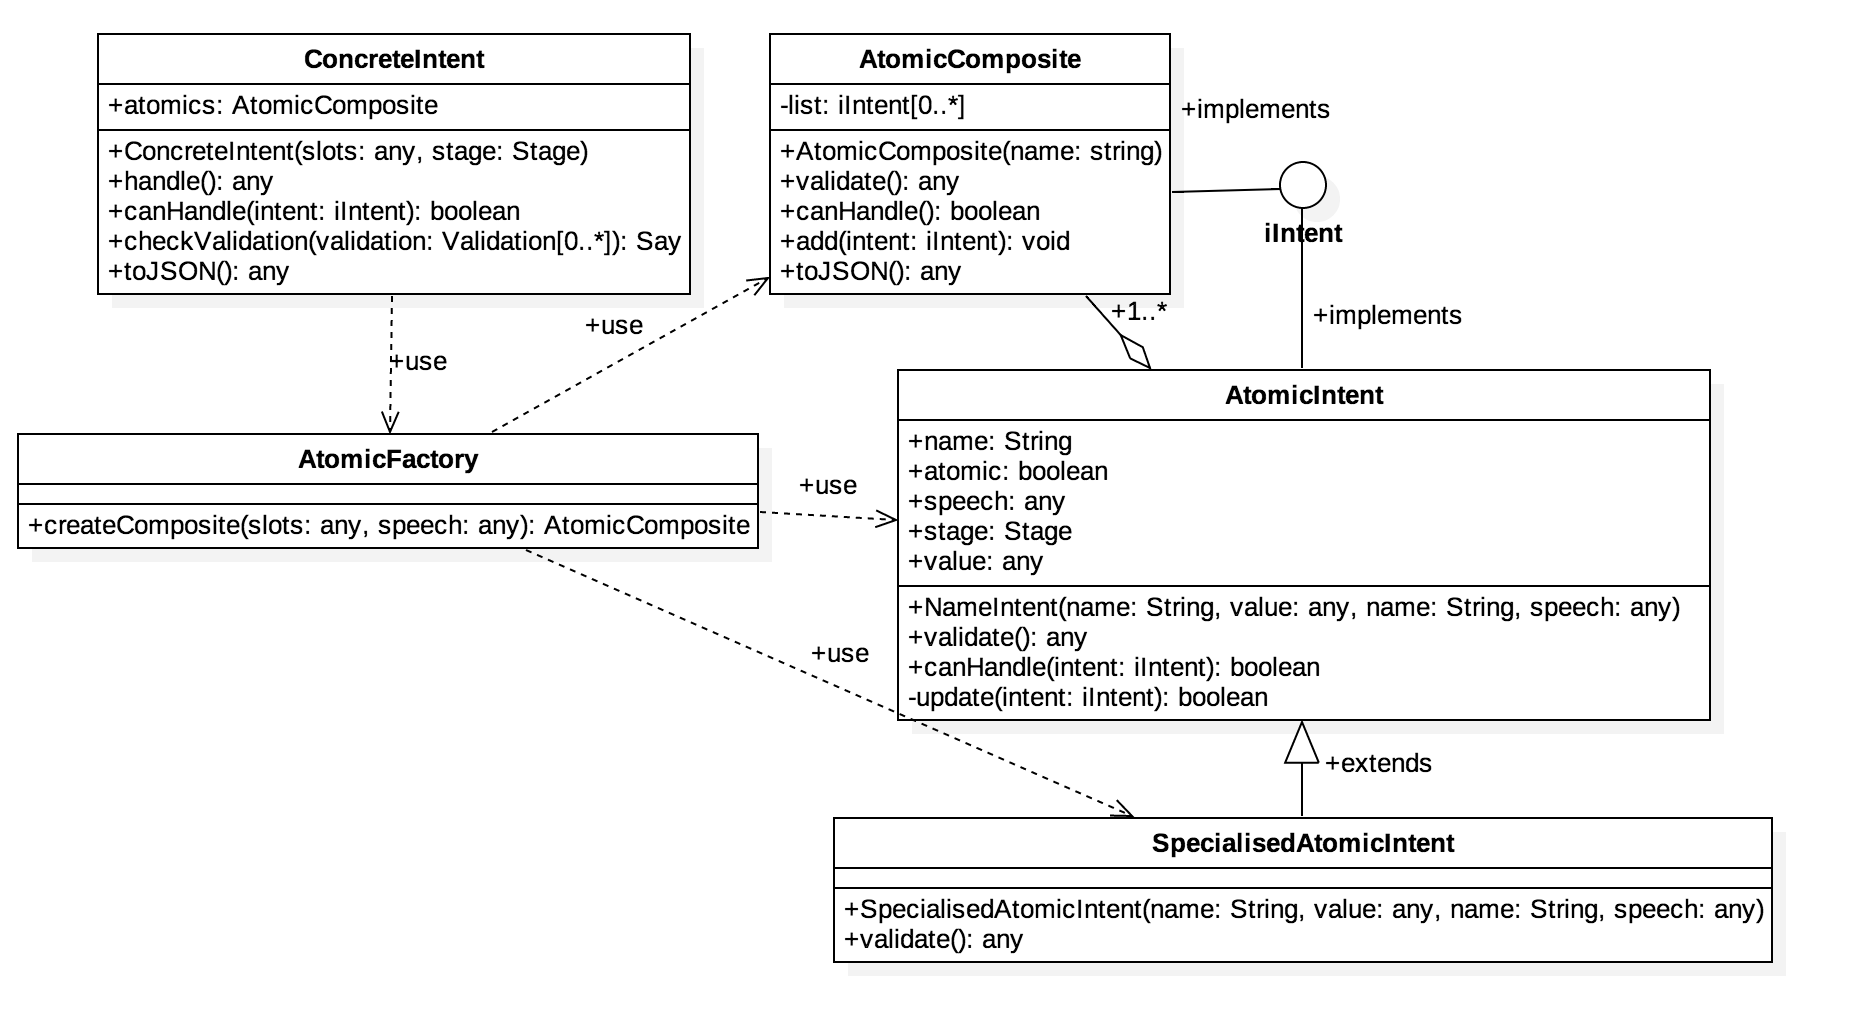
\includegraphics[width=1.0\textwidth]{bilder/4_klassenIntent.png}
    \caption{Vereinfachtes Klassendiagramm von Intent und Atomic Kompositum}
    \label{fig:skill-klassen-intent}
\end{figure}

Konkrete Intents, Atomic Intents und das Atomic Kompositum implementieren das iIntent Interface, dessen wichtigste Eigenschaften und Methoden vorerst erläutert werden.
\begin{itemize}
    \item \textit{atomic}: Legt fest \bzw zeigt an, ob es sich um einen Atomic Intent handelt oder nicht.
    
    \item \textit{speech}: Ein Objekt, dass die Antwortphrasen dieses Intents enthält. Konkrete Intents haben jeweils ein eigenes speech Objekt. 
    
    \item \textit{stage}: Die stage ist eine Enumeration, die verschiedene Stati beschreibt. Bei Atomic Intents dient der Status als Information, ob der Wert validiert wurde, fehlt oder vom Benutzer bestätigt werden muss. Andere Intents wie die Transaktion, die der Nutzer vor deren Durchführung ebenfalls bestätigen muss, greifen auch auf diese Eigenschaft zurück.
    
    \item \textit{value}: Der value ist optional, da er nur von Atomic Intents benötigt wird. Der value enthält den eigentlichen Wert, der über die Slots der Alexa Anfrage gesetzt wird. 
    
    \item \textit{validate()}: Diese Funktion bildet die Logik ab, mit der ein Atomic Intent validiert wird. Je nachdem was validiert werden muss, kann diese Logik variieren.
    
    \item \textit{handle()}: Diese Funktion enthält die Logik eines Intents.
    
    \item \textit{canHandle()}: Die canHandle Funktion wird beim Erstellen des Kontextes verwendet. Ist im Session-Objekt bereits ein Intent enthalten, wird geprüft, ob der Intent aus der Anfrage von diesem gehandhabt werden kann. Ein Beispiel soll dies verdeutlichen. Ein Benutzer hat eine Transaktion angestoßen, jedoch vergessen den Betrag zu nennen. Die Transaktion wird mit dem aktuellen Stand in das Session-Objekt gespeichert. Der Benutzer erhält die Antwort, dass der Betrag fehlt. Spricht der Benutzer nun eine Nummer in den Echo wird dabei der Atomic Intent „Number“ adressiert. Im Kontext wird nun geprüft ob der Transaktions Intent den Number Intent handhaben kann. Da dies der Fall ist, wird der Betrag des Transaktions Intent mit dem Wert des Number Intents aktualisiert.
\end{itemize}

Beim Erstellen eines konkreten Intents wird die Alexa Request an die Intent Factory übergeben. Falls Slots für diesen Intent vorgesehen sind, übergibt die Factory die Daten entsprechend. Innerhalb des konkreten Intent Konstruktors wird eine weitere Factory verwendet, um das Atomic Kompositum aufzubauen. Die Atomic Factory instanziiert ein solches Kompositum und fügt für jeden übergebenen Slot den entsprechenden Atomic Intent hinzu. Aufgrund der Implementierung des iIntent Interfaces, kann das Kompositum von außen als ein Intent Objekt und nicht als Liste behandelt werden. Es spielt dabei keine Rolle ob es nur einen oder viele Atomic Intents enthält. Abbildung \ref{fig:skill-sequenz-kompositum} zeigt das entsprechende Sequenzdiagramm. Es verdeutlicht die Schritte zwischen Sequenz 4 und 5 des Diagrammes aus Abbildung \ref{fig:skill-sequenz-kontext}.\newpage

\begin{figure}[!htb]
    \centering
    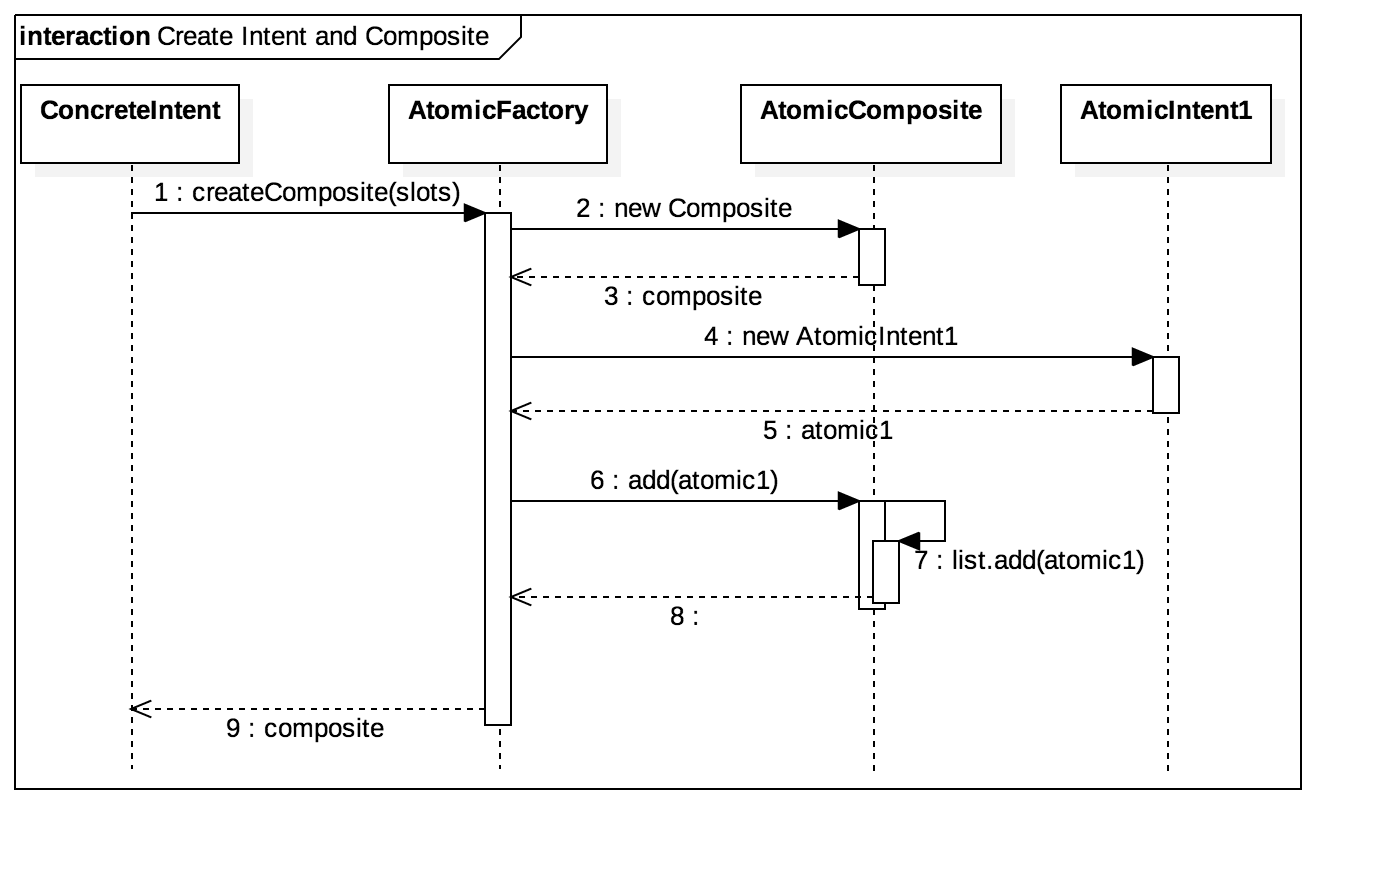
\includegraphics[width=1.0\textwidth]{bilder/4_skillSequenzIntentKompositum.png}
    \caption{Sequenzdiagramm Instanziierung eines Atomic Kompositums}
    \label{fig:skill-sequenz-kompositum}
\end{figure}

Nun sollen die Prozesse zwischen den Schritten 10 und 11 aus dem Sequenzdiagramm in Abbildung \ref{fig:skill-sequenz-kontext} beschrieben werden. Dabei handelt es sich um die Logik \bzw handle Funktion eines konrekten Intents. An dieser Stelle muss man zwischen Intents mit und ohne Slots \bzw Kompositum unterscheiden. Der „Hilfe“ Intent, der keine Slots enthält, gibt lediglich eine der vordefinierten Antworten aus. Sind Slots vorhanden, unterscheiden sich die Methoden je nach Anwendungsfall, dennoch ist ihr grundlegender Aufbau identisch. Zunächst wird die „validate“ Funktion des Kompositums ausgeführt. Sequentiell werden die Ergebnisse jedes Atomic Intents in Form von „Validation“ Objekten einer Liste hinzugefügt, welche zurück an den Intent geht. Diese Objekte umfassen jeweils die Antwortphrase und Stage eines Atomic Intents. Zurück im Intent setzt die „checkValidation“ Methode aus dieser Liste eine Antwort zusammen. Ist die Antwort leer, sind alle Atomic Intents erfolgreich validiert und die handle Logik kann weiter ausgeführt werden. Das Programm holt beispielsweise Daten vom Backend, generiert eine Antwort und gibt diese zurück. Für den Fall, dass die Antwort aus der checkValidation Methode nicht leer ist, beinhaltet sie weitere Rückfragen an den Benutzer. Dabei wird sie direkt und ohne Ausführung der weiteren Logik, an diesen zurückgegeben. Bei den Rückfragen kann es sich um fehlende Slots handeln, die noch eingegeben werden müssen. Falls nötig, wird vor dem Zurückgeben der Antwort der Session Kontext auf den aktuellen Stand gesetzt. Das ist vor allem bei fehlenden Slots der Fall. Diese werden zusammen mit ihren Werten und Stages im Session-Objekt unter dem entsprechenden Intent Namen gespeichert. Stößt der Benutzer den nächsten Schritt der Konversation an, kann der gespeicherte Intent ausgewertet und im neuen Kontext verwendet werden.  Abbildung \ref{fig:skill-sequenz-handle} zeigt die Prozesse der Intent Logik in einem Sequenzdiagramm .

\begin{figure}[!htb]
    \centering
    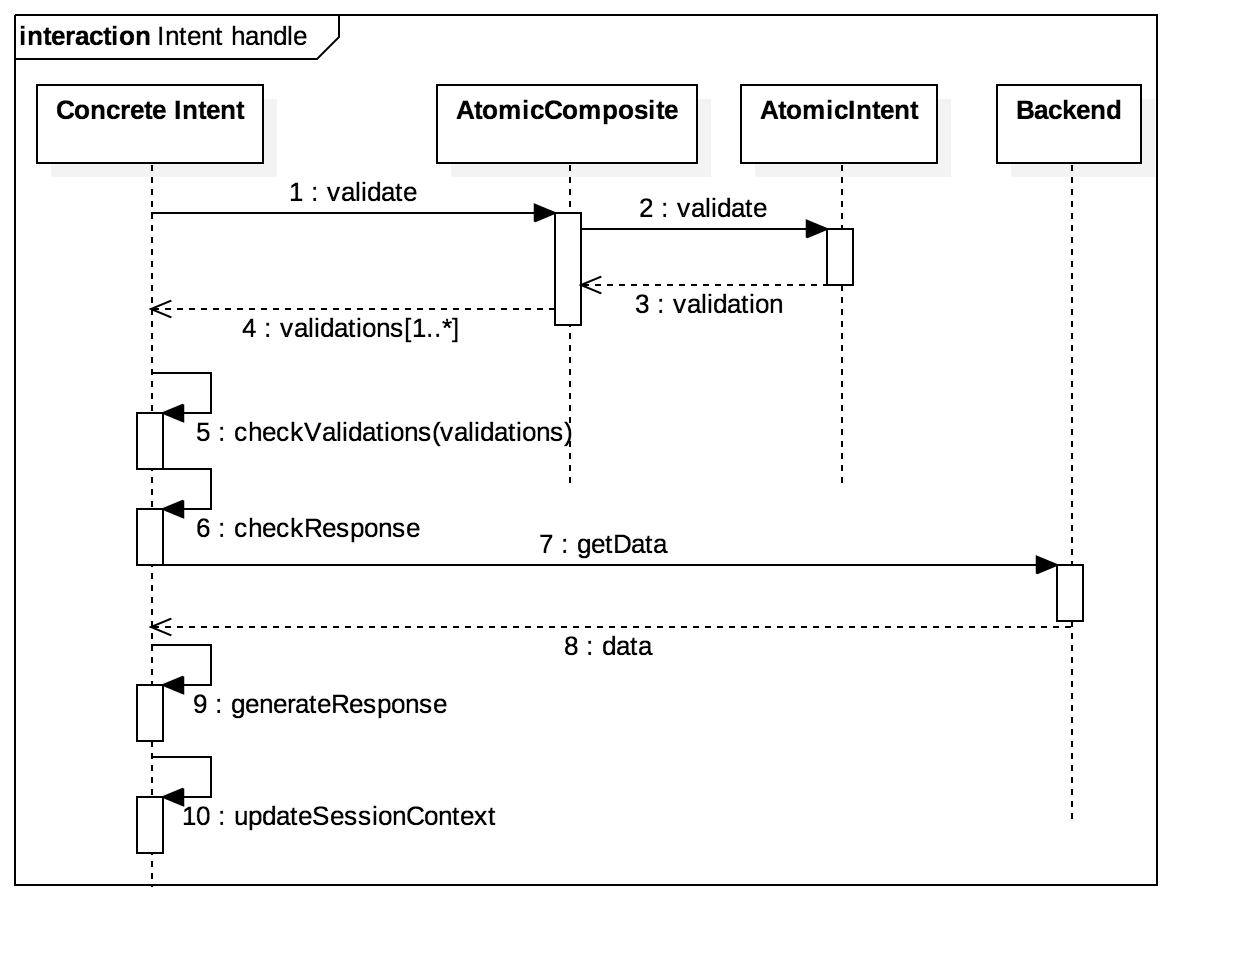
\includegraphics[width=1.0\textwidth]{bilder/4_skillSequenzIntentHandle.png}
    \caption{Sequenzdiagramm der Intent handle Funktion}
    \label{fig:skill-sequenz-handle}
\end{figure}

Die hier gegebenen Beschreibungen stellen die Prozesse der Architektur in allgemeiner Form dar. Im Folgenden werden daher die implementierten Intents mit ihren Besonderheiten zusammengefasst. 

\begin{itemize}
    \item Launch Intent: Der Launch Intent wird ausgeführt, wenn ein Benutzer den Skill startet und gibt lediglich eine der vordefinierten Antworten aus, um den Benutzer zu begrüßen. Dabei handelt es sich um einen Standard Intent, den jeder Skill implementieren muss
    
    \item Stop Intent: Mit dem Stop Intent verabschiedet sich der Skill vom Benutzer und beendet sich. Dieser Intent ist ebenfalls vorgeschrieben und muss von Skills implementiert werden.
    
    \item Help Intent: Auch die Hilfe muss implementiert werden. Sie gibt Beispielphrasen aus, die Nutzer für die Interaktion mit dem Skill verwenden können.
    
    \item User Intent: Der User Intent wird verwendet, um den Namen des Benutzers in Erfahrung zu bringen. Dabei handelt es sich um einen besonderen Intent. Er wird nicht vom Benutzer angestoßen, sondern in bestimmten Fällen vom Programm als Kontext im Session-Objekt gesetzt. Das ist notwendig, damit ein anschließend eingegebener Name auch als Benutzer Name für die Authentifizierung interpretiert werden kann. Ein Beispiel ist der Launch Intent. Nach Ausgabe des Willkommens Grußes, erfragt der Skill den Benutzer Namen. Ein weiteres Beispiel sind die Banking Funktionen. Ist der Benutzer bei Abfrage des Kontostandes noch nicht identifiziert, setzt der Skill den User Intent als Kontext und bittet den Benutzer  seinen Namen zu nennen. Nach Eingabe wird der Authentifizierungsmechanismus aus Abbildung \ref{fig:sequenz-authentifizierung} angestoßen.
    
    \item Authorise Intent: Ähnlich wie der User Intent, wird der Authorise Intent in bestimmten Situationen vom Programm initiiert. Er wird verwendet wenn ein bekannter, jedoch noch nicht authentifizierter Benutzer Banking Funktionen nutzen möchte. Über den Authorise Intent wird dann eine erneute Push-Nachricht an das Smartphone des Nutzers geschickt, damit dieser per Fingerabdruck bestätigt. 
    
    \item Balance Intent: Der Kontostand Intent enthält keine Slots. Wie im Authorise Intent beschrieben müssen Benutzer authentifiziert sein, bevor eine Abfrage des Kontostandes möglich ist. Natürlich muss der Benutzer vorher ein Konto über die App anbinden, um diese Funktion zu nutzen. Gemäß Abbildung \ref{fig:sequenz-kontostand} wird der Kontostand über das Backend und den Multibanking-Mock erfragt. 
    
    \item Transaction Intent: Die Transaktion ist der komplizierteste der implementierten Intents. Auch hier müssen zunächst Kriterien erfüllt werden. Ein Benutzer muss authentifiziert sein, ein Konto angebunden und Überweisungsvorlagen erstellt haben. Die Vorlage und der Betrag müssen vom Benutzer eingegeben werden. Bei fehlenden Slots gibt der Skill entsprechende Rückfragen aus. Ist die Validierung erfolgreich, wird die Überweisung zur Bestätigung noch einmal ausgegeben. Die Transaktion wird als Kontext gesetzt. Der Benutzer kann nun mit „ja“ bestätigen oder mit „nein“ ablehnen. Dabei handelt es sich auch um Atomic Intents. Ein „ja“ legt die Transaktion an. Der \ac{TAN} wird an das Smartphone des Benutzers gesendet. Im Anschluss setzt der Skill den \ac{TAN} Intent als Kontext. Bei einem „nein“ kann der der Benutzer die Slots noch einmal ändern oder andere Funktionen nutzen.
    
    \item \ac{TAN} Intent: Beim \ac{TAN} handelt es sich ebenfalls um einen vom Skill initiierten Intent. Nach Anlegen einer Transaktion wird dieser als Kontext gesetzt. Die an das Benutzer Smartphone übermittelte Nummer kann nun über Alexa eingegeben werden. Stimmt die Nummer überein, wird die Transaktion durchgeführt. Im Fehlerfall wird eine entsprechende Antwort ausgegeben.
\end{itemize}

An dieser Stelle sei erwähnt, dass der Kontext \bzw der aktuelle Intent jederzeit gewechselt werden kann. Auch wenn der Skill den Benutzer darum bittet die \ac{TAN} einer Überweisung einzugeben, kann dieser im nächsten Schritt den Hilfe- oder Kontostand Intent ansprechen. Mit dem entwickelten Prototypen ist es allerdings nicht möglich, im Anschluss zurück zum \ac{TAN} Intent zu wechseln. Auch wenn dies technisch möglich ist, kann es aus zeitlichen Gründen nicht im Zuge dieser Arbeit umgesetzt werden.\\
Damit Alexa die Daten entsprechend der Implementierung verstehen und an den Skill-Server senden kann, wird in Kapitel \ref{sec:interaction-model} das Interaction Model des Skills erstellt. Der Quelltext des Voice Bank Skill-Servers ist auf der beiliegenden CD unter \textit{„Quelltexte/finlexa\_skill/“} zu finden.

\section{Interaction Model}
\label{sec:interaction-model}
Damit Alexa die verwendeten Formulierungen für den Skill verstehen kann, muss man das Interaction Model erstellen. Hier werden die Intens, Slots und Utterances des Skills angegeben und miteinander verknüpft. Dabei wird das Konzept aus Kapitel \ref{sec:anhang-konzept} für die implementierten Intents verwendet. Des Weiteren sind hier der Skill und Invocation Name einzutragen.  Abbildung \ref{fig:interaction-model} zeigt den Abschnitt des Amazon Developer Portals, der für das Interaction Model des Voice Bank Skill zuständig ist. \newpage

\begin{figure}[!htb]
    \centering
    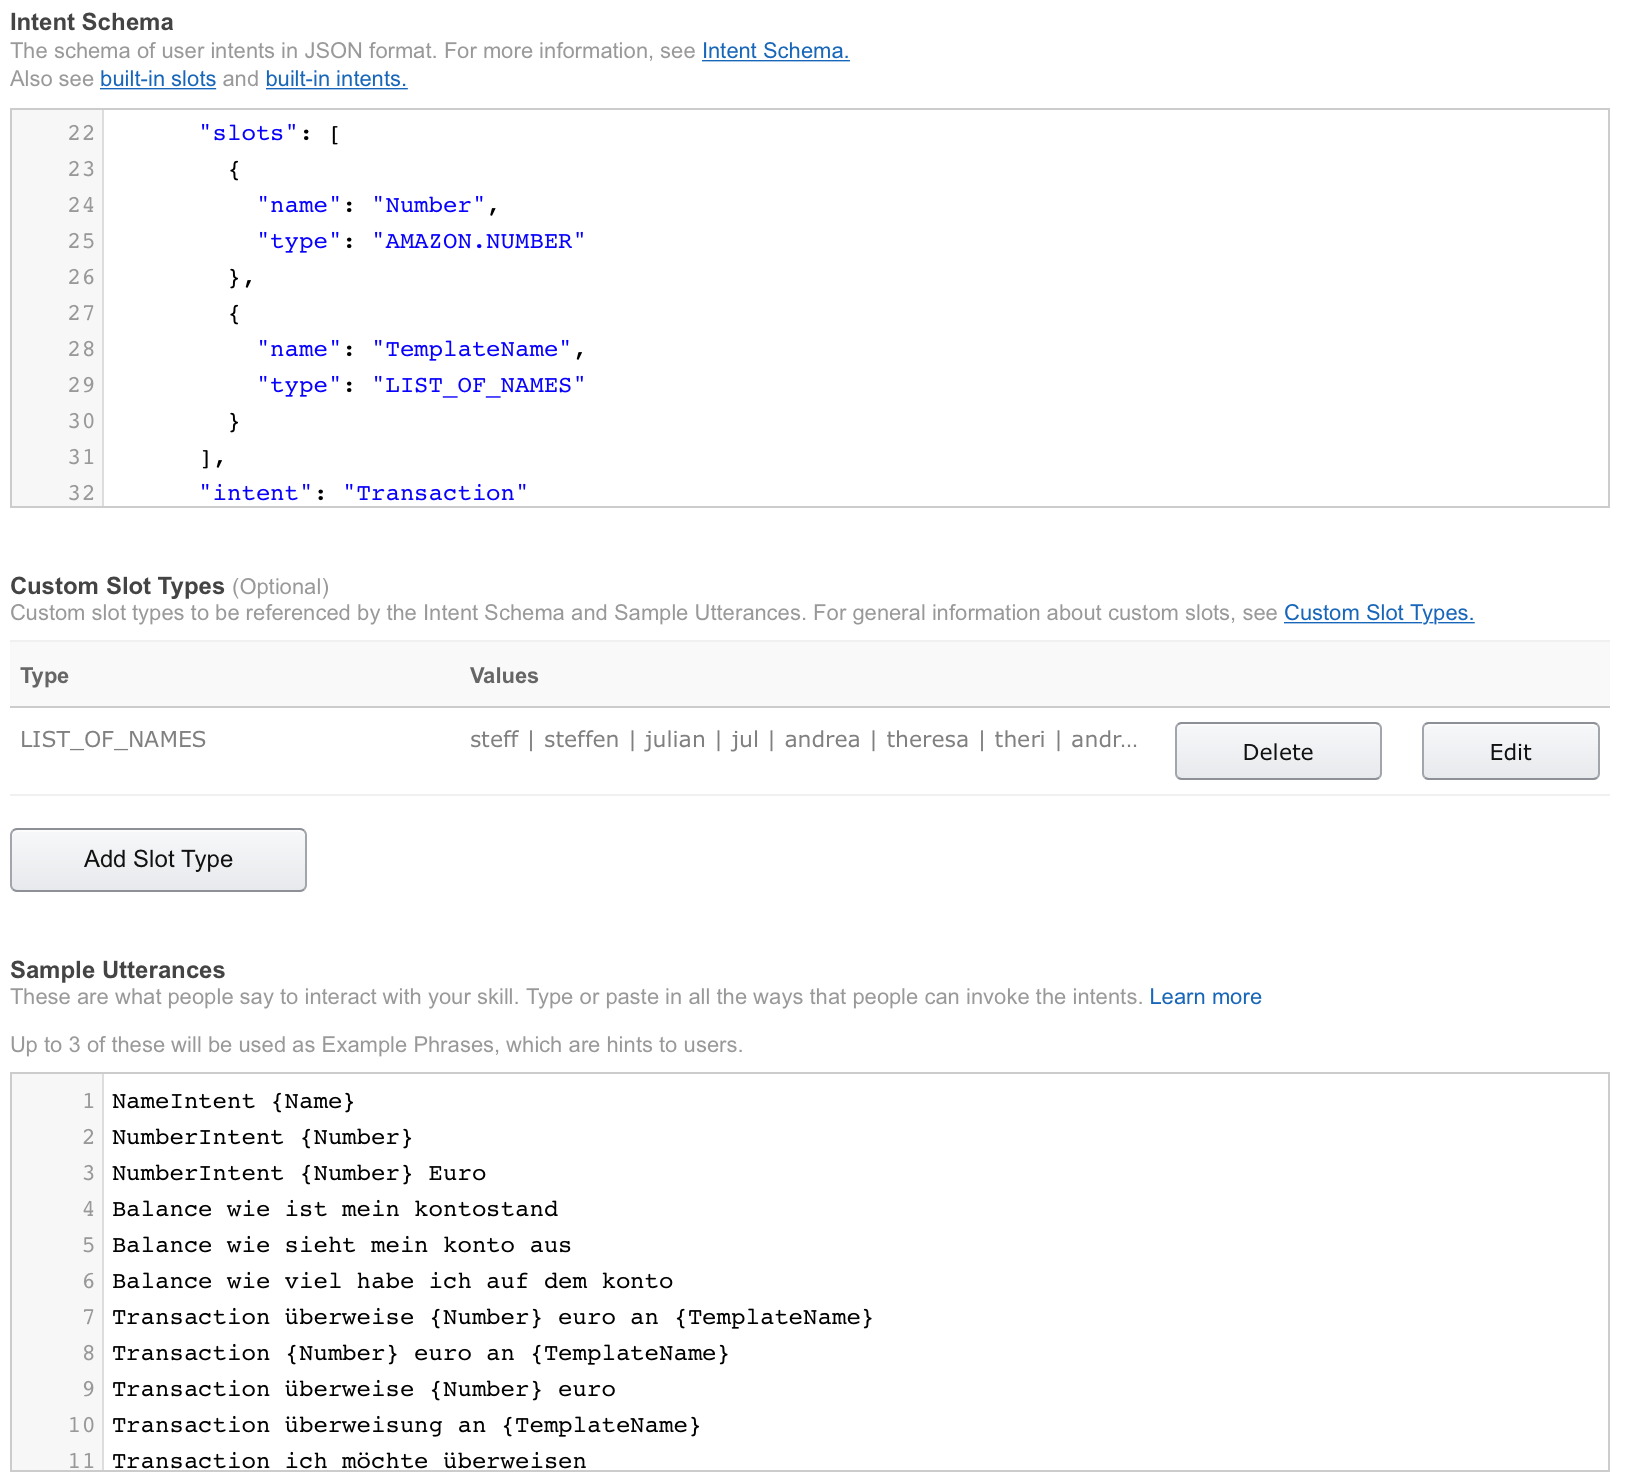
\includegraphics[width=1.0\textwidth]{bilder/4_interactionModel.png}
    \caption{Ausschnitt des Voice Bank Interaction Models}
    \label{fig:interaction-model}
\end{figure}

Dort sind das \textit{Intent Schema}, \textit{Custom Slot Values} und die Utterances zu sehen. Im Intent Schema wird zunächst jeder verwendete Intent mit etwaigen Slots in \ac{JSON} Form angegeben. Neben den Slot Namen ist hier auch der Typ festzulegen. Amazon unterstützt häufig verwendete Typen wie \zB \textit{AMAZON.Date}, \textit{AMAZON.Number} und \textit{AMAZON.Time} \cite{alexa-slot-types}. Diese ermöglichen, dass selbst unterschiedlich formulierte Eingaben eine einheitliche Ausgabe für den Skill-Server gewährleisten. Angaben zu einem bestimmten Tag, darunter „morgen“, „Dienstag“ oder „22.11.2017“, werden in Form von „YYYY-MM-DD“ ausgegeben, \zB 2017-11-22. Während Eingaben zu Wochen, wie „diese Woche“ und “nächste Woche“, als Kalenderwoche interpretiert werden \zB 2017-W47. Es ist auch möglich eigene Typen zu definieren. Das sind die Custom Slot Values aus Abbildung \ref{sec:interaction-model}. Im unteren Feld werden die Utterances nach dem bereits bekannten Schema (\vgl Kapitel \ref{subsec:skill-ask-sdk} und \ref{subsec:skill-architektur}) eingetragen. Abbildung \ref{sec:interaction-model} zeigt dabei nur einen Ausschnitt der definierten Formulierungen. Hier zu sehen sind die zwei Atomic Intents „Number“, “Name“ und ein Teil der „Kontostand“ und “Transaktion“ Intents. An dieser Stelle fließen auch die erarbeiteten Formulierungen aus dem Konzept mit ein. Sämtliche Utterances aus Abbildung \ref{fig:concept-transaction-name} und \ref{fig:concept-balance} werden ergänzt. Im nächsten Schritt ist die Adresse des Skill-Servers zu konfigurieren. Diese wird in Kapitel \ref{sec:deployment} eingefügt, da der Server zunächst bereitgestellt werden soll. Mit dem Anlegen dieses Skills im Developer Portal, der Angabe des Invocation \bzw Skill Namens, des Models und der Server Adresse kann der Skill bereits mit den Alexa Endgeräten des Entwicklers genutzt werden. Um den Skill in den Store hochzuladen, damit ihn auch andere Benutzer verwenden können, sind weitere Schritte nötig. Dabei müssen eine Beschreibung, Beispielphrasen für die Verwendung, ein Icon und weitere Angaben gemacht werden. Der Prozess der Skill Veröffentlichung wird im Zuge dieser Arbeit nicht beschrieben. Das Intent Schema und die Utterances des Interaction Models sind auf der CD unter \textit{„Quelltexte/finlexa\_model“} zu finden. Kapitel \ref{sec:deployment} zeigt den Vorgang und die verwendeten Technologien bei der Bereitstellung des Skill-Servers und Backends.

\section{Deployment}
\label{sec:deployment}
Der umgesetzte Prototyp wird nicht nur lokal über den Rechner gestartet. Der Skill-Server ist über das Web erreichbar. Dabei kommt nicht \ac{AWS}, sondern die Infrastruktur des Projektträgers zum Einsatz. Die dabei verwendeten Technologien werden im Folgenden kurz zusammengefasst.

\begin{itemize}
    \item \textit{Docker}: Docker ist eine offene Plattform zum Entwickeln, Ausliefern und Betreiben von verteilten Applikationen. Anwendungen sind in unabhängigen Containern organisiert. Anders als eine \ac{VM}, nutzen Docker Container das vorhandene Betriebssystem. Das spart Rechenleistung, da kein zusätzliches Betriebssystem emuliert werden muss. Über eine entsprechende Konfigurationsdatei kann mit Hilfe der Kommandozeile ein Abbild eines Containers generiert und gestartet werden. Diese können auch auf Server und Cloud Plattformen hochgeladen werden \cite{docker}. Listing \ref{lst:dockerfile} zeigt die Konfigurationsdatei, das sogenanntes \textit{dockerfile}, für den Skill-Server.\newpage
    
    \begin{lstlisting}[language={HTML},caption={Dockerfile des Voice Bank Skill-Servers},label={lst:dockerfile}]
    FROM node:boron

    ADD . /usr/src/app
    WORKDIR /usr/src/app
    
    RUN npm install -g tsc typescript
    
    RUN npm install
    
    RUN tsc 
    
    EXPOSE 3000
    CMD ["npm", "start"]

    \end{lstlisting}
    
    Dabei wird ein Basis Container „node:boron“ verwendet, der auf einem Linux Betriebssystem aufsetzt und bereits Node.js vorinstalliert hat. Im Anschluss werden die relevanten Quelltext Dateien (hier TypeScript Code) des Skill-Servers in die Ordnerstruktur der Linux Umgebung kopiert. Benötigte \ac{npm} Module müssen zunächst installiert werden. Im weiteren Verlauf wird der \ac{TS} Code kompiliert, der Port 3000 freigegeben und die Anwendung gestartet.
    
    \item \textit{OpenShift}: OpenShift ist eine open source Container Plattform. Sie basiert \ua auf Docker und ermöglicht das Verwalten, Betreiben und Warten von Docker Containern in Projekten. Ein Projekt kann dabei mehrere Container enthalten, die untereinander kommunizieren und von außen erreichbar sein können. Die OpenShift Umgebung wird vom Projektträger bereit gestellt. 
\end{itemize}

Skill-Server, Backend und die Datenbank sind jeweils in einem eigenen Docker Container organisiert. Die entsprechenden dockerfiles sind auf der CD im jeweiligen Ordner abgelegt. Das Dockerfile der Datenbank befindet sich unter \textit{„Quelltexte/finlexa\_central/database/“}. Diese Container werden in ein Projekt auf der OpenShift Plattform des Projektträgers hochgeladen. Abbildung \ref{fig:openshift} zeigt die Web Oberfläche dieses Projektes mit den drei laufenden Containern.\newpage

\begin{figure}[!htb]
    \centering
    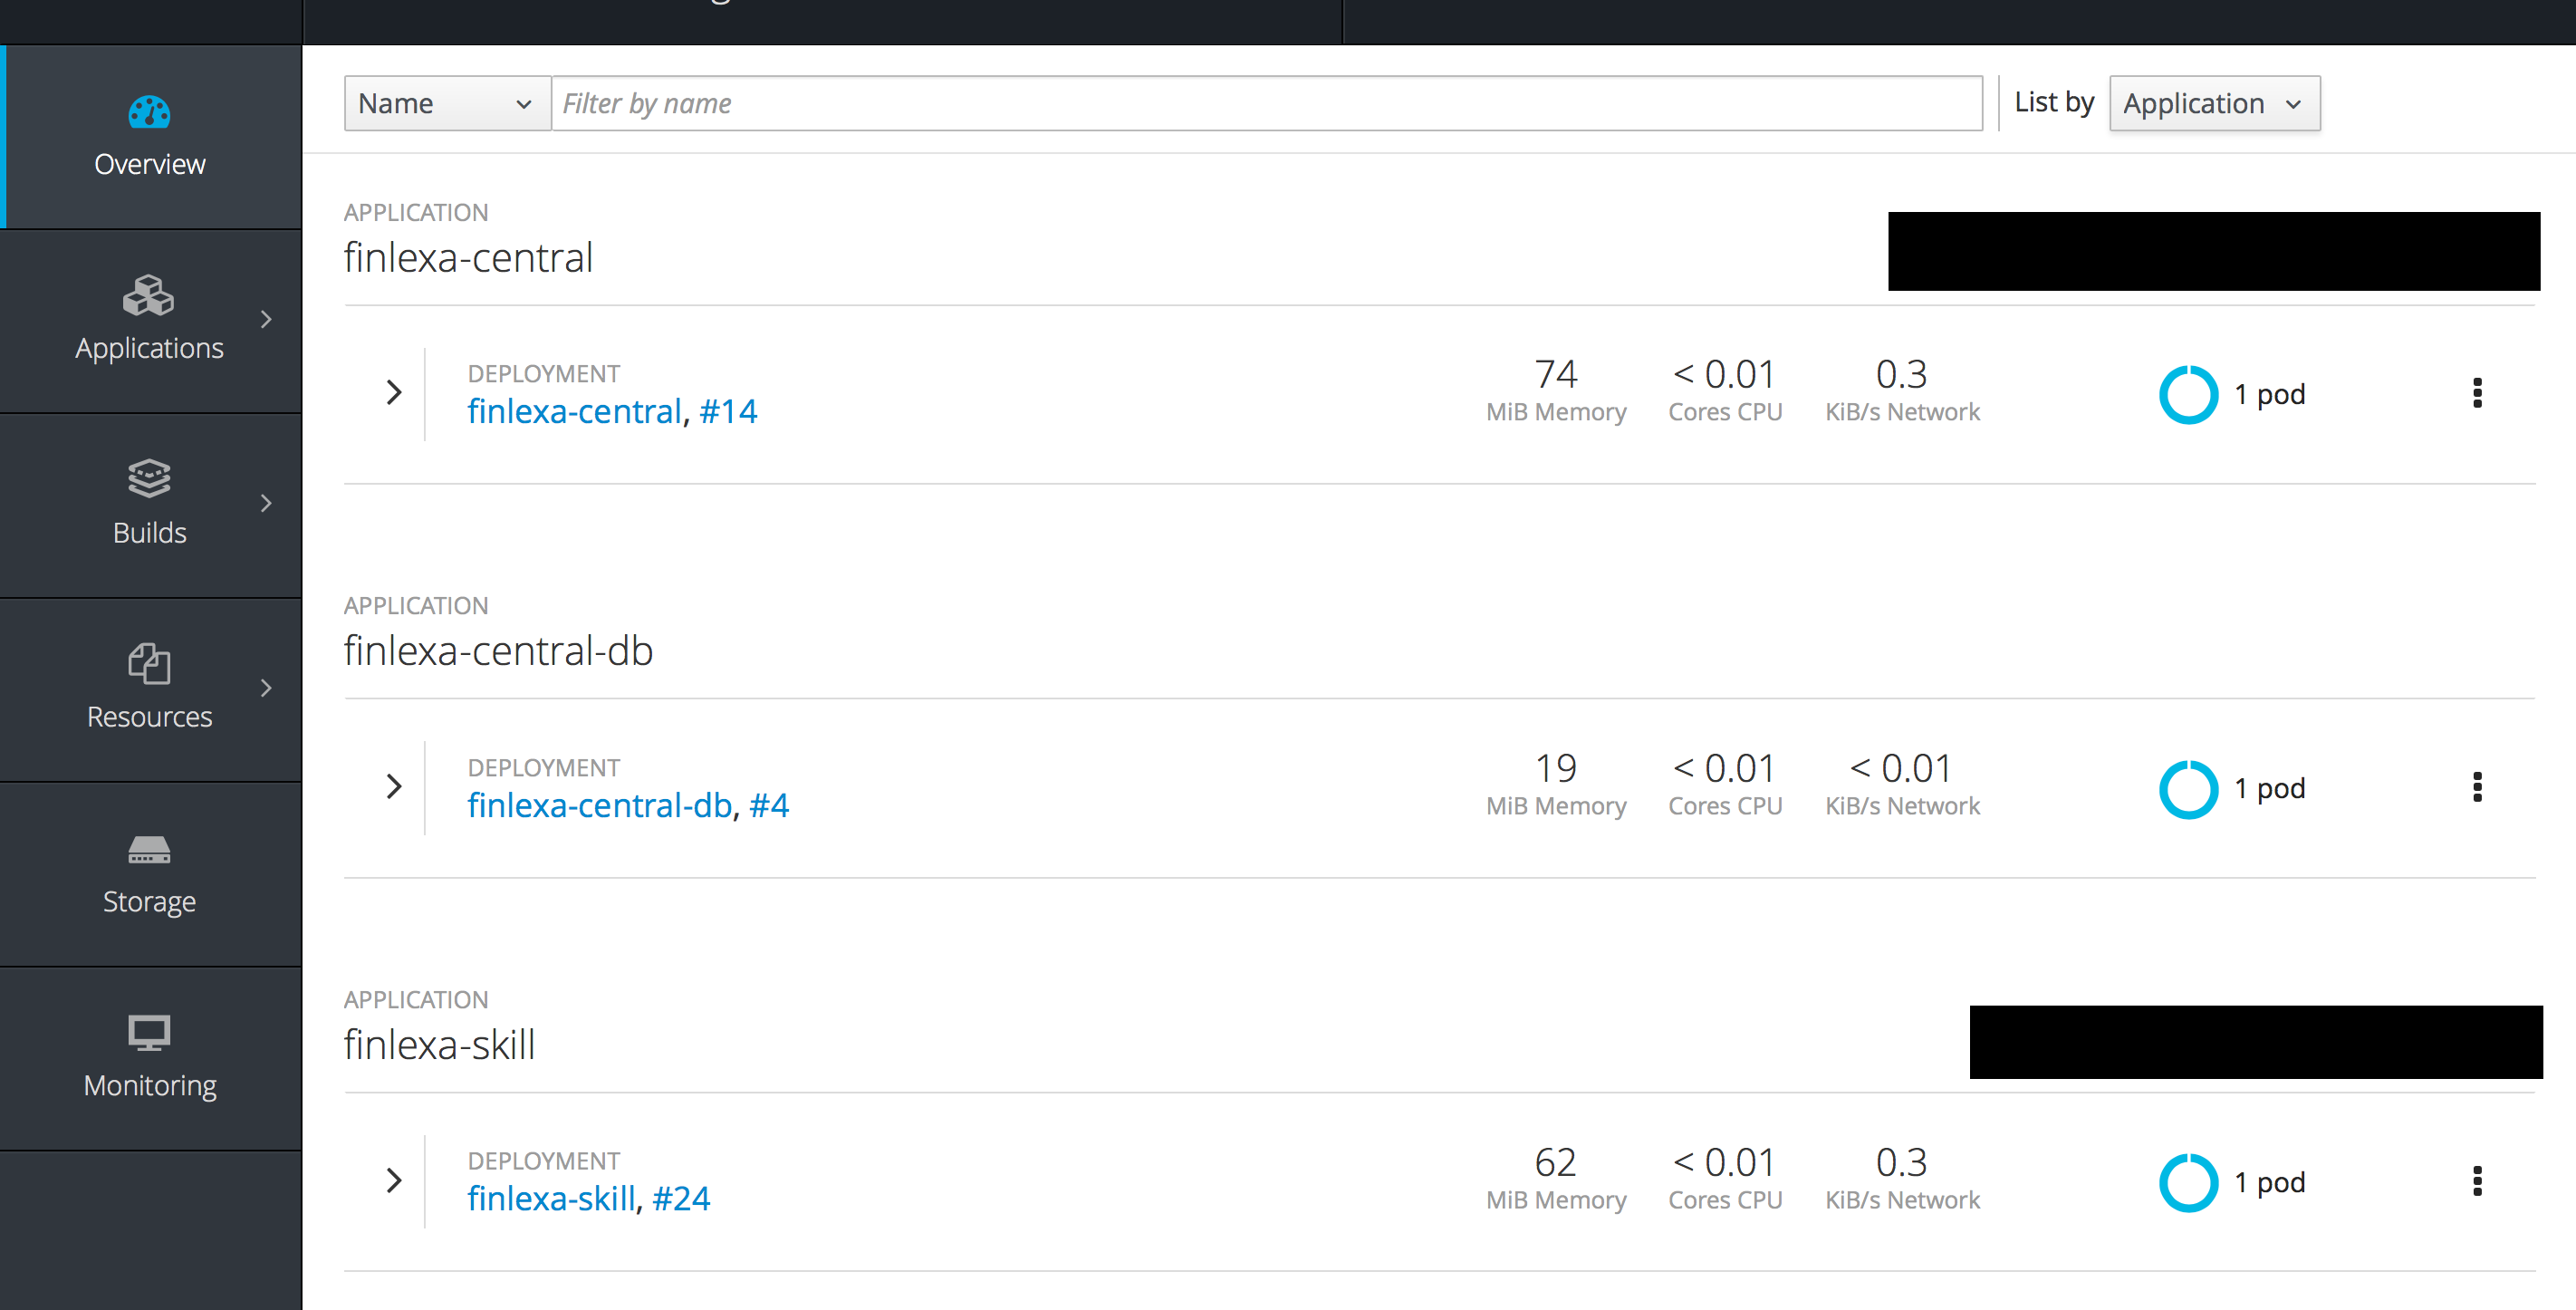
\includegraphics[width=1.0\textwidth]{bilder/4_openshift.png}
    \caption{Voice Bank Projekt in OpenShift}
    \label{fig:openshift}
\end{figure}

Da der Name des Systems erst gegen Ende der Arbeit von „finlexa“ auf „Voice Bank“ geändert wurde, sind die Container hier mit dem alten Namen gekennzeichnet. Der „finlexa-central“ bildet das in der Umsetzung beschriebene Backend ab. Damit der Skill-Server und das Backend von außen erreichbar sind, werden für beide Routen angelegt. Die entsprechenden \acp{URL} sind in Abbildung \ref{fig:openshift} aus Sicherheitsgründen geschwärzt. Wird im Interaction Model die hier angelegte Route als Adresse des Skill-Servers eingegeben, hat Alexa Zugriff und der Skill kann über den Echo verwendet werden. Ebenso muss die Adresse des Backends in der Smartphone-App hinterlegt sein. Das folgende Kapitel \ref{sec:evaluierung} evaluiert die beschriebene Umsetzung des Prototypen.

\section{Evaluierung}
\label{sec:evaluierung}
Nach ersten Konversationen mit dem Skill Prototypen, wird klar, dass das kontextbasierte Verarbeiten der Intents, Komplettieren der Slots und die Authentifizierung den konzipierten Sequenzen folgen. Anhand dessen kann man darauf schließen, dass das Sicherheits-Konzept und die implementierte Architektur funktionieren. Es sei jedoch an dieser Stelle erwähnt, dass aufgrund der zeitlichen Begrenzung keine User Tests mit dem Prototypen durchgeführt werden können. Da die entwickelte App (Kapitel \ref{sec:app}) aus dem gleichen Grund eher funktional und weniger benutzerfreundlich umgesetzt ist, hat sie beim Test des Gesamtsystems womöglich negative Auswirkungen. Um zu beweisen, dass das System auch zufriedenstellend funktioniert und um eine fundierte Aussage treffen zu können, muss demnach die App entsprechend entwickelt und der Skill außerhalb dieser Arbeit getestet werden.\\ 
Die Implementierung der Architektur an sich ist anfangs zeitaufwändig. Jedoch ist zu bemerken, dass die Stärken vor allem bei zunehmender Komplexität ersichtlich werden. Hat man das Grundgerüst programmiert, lassen sich neue Intents \bzw Atomic Intents schnell hinzufügen. Aufgrund der Klassenhierarchie sind lediglich die Routinen der Valdierung \bzw handle Methode zu schreiben, die Intents in die entsprechende Fatory einzupflegen und die Antwortphrasen zu definieren. Das umgesetzte Sicherheits-Konzept zeigt außerdem, dass die Interaktion zwischen Alexa und der entwickelten App auch ohne Event-Unterstützung erfolgen kann. Es bietet die Möglichkeit Benutzer ohne Stimmenerkennung zu identifizieren. Jedoch ist die Nutzung des Mechanismus mit mehr Zeitaufwand für den Nutzer verbunden. Das folgende Kapitel \ref{cha:schlussbetrachtung} zieht ein Fazit der gesamten Arbeit und gibt einen Ausblick.

